\documentclass{article}



\usepackage{arxiv}

\usepackage[utf8]{inputenc} % allow utf-8 input
\usepackage[T1]{fontenc}    % use 8-bit T1 fonts
\usepackage{hyperref}       % hyperlinks
\usepackage{url}            % simple URL typesetting
\usepackage{booktabs}       % professional-quality tables
\usepackage{amsfonts}       % blackboard math symbols
\usepackage{nicefrac}       % compact symbols for 1/2, etc.
\usepackage{microtype}      % microtypography
\usepackage{lipsum}		% Can be removed after putting your text content
\usepackage{graphicx}
\usepackage{natbib}
\usepackage{doi}

\usepackage[dvipsnames]{xcolor}
\newcommand{\andy}[1]{\textcolor{blue}{\emph{#1}}}

\title{Could mass eccentricity explain the formation of orbits in wind turbines?}

%\date{September 9, 1985}	% Here you can change the date presented in the paper title
%\date{} 					% Or removing it

\author{ \href{https://orcid.org/0000-0001-8717-9688}{
\includegraphics[scale=0.06]{orcid.pdf}\hspace{1mm} Aljoscha Sander} \\
	Energy and Sustainability Research Institute Groningen\\
	University of Groningen\\
	Groningen, the Netherlands \\
	\texttt{aljoscha.sander@rug.nl} \\
	%% examples of more authors
	\And
	\href{https://orcid.org/0000-0000-0000-0000}{
\includegraphics[scale=0.06]{orcid.pdf}\hspace{1mm} Andreas Haselsteiner} \\
	\texttt{a.haselsteiner@uni-bremen.de} \\
	\And
	Bas Holman \\
	\texttt{b.holman@outlook.com}\\
	%% Address \\
	%% \texttt{email} \\
	%% \And
	%% Coauthor \\
	%% Affiliation \\
	%% Address \\
	%% \texttt{email} \\
	%% \And
	%% Coauthor \\
	%% Affiliation \\
	%% Address \\
	%% \texttt{email} \\
}

% Uncomment to remove the date
%\date{}

% Uncomment to override  the `A preprint' in the header
%\renewcommand{\headeright}{Technical Report}
%\renewcommand{\undertitle}{Technical Report}
\renewcommand{\shorttitle}{Mass eccentricity in offshore wind turbines}

%%% Add PDF metadata to help others organize their library
%%% Once the PDF is generated, you can check the metadata with
%%% $ pdfinfo template.pdf
\hypersetup{
pdftitle={Could mass eccentricity explain the formation of orbits in wind turbines?},
pdfsubject={},
pdfauthor={Aljoscha Sander, Andreas Haselsteiner, Bas Holman},
pdfkeywords={First keyword, Second keyword, More},
}

\begin{document}
\maketitle

\begin{abstract}
\end{abstract}


% keywords can be removed
\keywords{First keyword \and Second keyword \and More}


\section{Introduction}
\label{sec:introduction}

Offshore wind is growing continuously and is on its way to become one of the pillars of green energy. Recent cost reductions in offshore wind (29 \%) have mostly been due to increasing turbine size \citep{irenaRenewablePowerGeneration2020}. Increasing turbine size and numbers, however, leads to increasing difficulties during installation: larger components are more difficult to handle and require more space on an installation vessel. Today, most turbines are installed component by component, including the blades, a process generally referred to as single blade installation \citep{jiangInstallationOffshoreWind2021}. Blades are installed utilizing a specialized tool, usually referred to as an installation yoke, that securely fastens the blade during craning operations. Once the blade reaches hub height, a guiding pin is used to land the blade's bolts in the corresponding holes in the rotor flange. During this operation, relative motion between the blade root and the rotor hub greatly hampers the secure landing of the blade in the rotor's flange. As these relative motions are driven by environmental loading on both the turbine and the blade, they are difficult to understand and even more so to predict. 

In a measurement campaign conducted during the installation of the offshore wind farm \textit{Trianel Windpark Borkum II} off the coast of Germany in the German Bight, the kinematics of blades and partially installed turbines were investigated \citep{sanderRelativeMotionSingle2020,  sanderMONITORINGOFFSHOREWIND2020, sanderOscillationsOffshoreWind2020}. These measurements revealed, that the partially installed turbines were displaying intricate patterns of motions — orbits — during single blade installation. A two-minute orbit captured during the installation of the wind park \textit{Trianel Windpark Borkum II} is shown in \autoref{fig:orbit}. These orbits show that amplitude and direction of tower top motion may appear swiftly and with large rates of change. It stands to reason that these orbits in turn influence the installation of blades and may even be responsible for an increase in installation difficulty.

\begin{figure}[ht!]
    \centering
    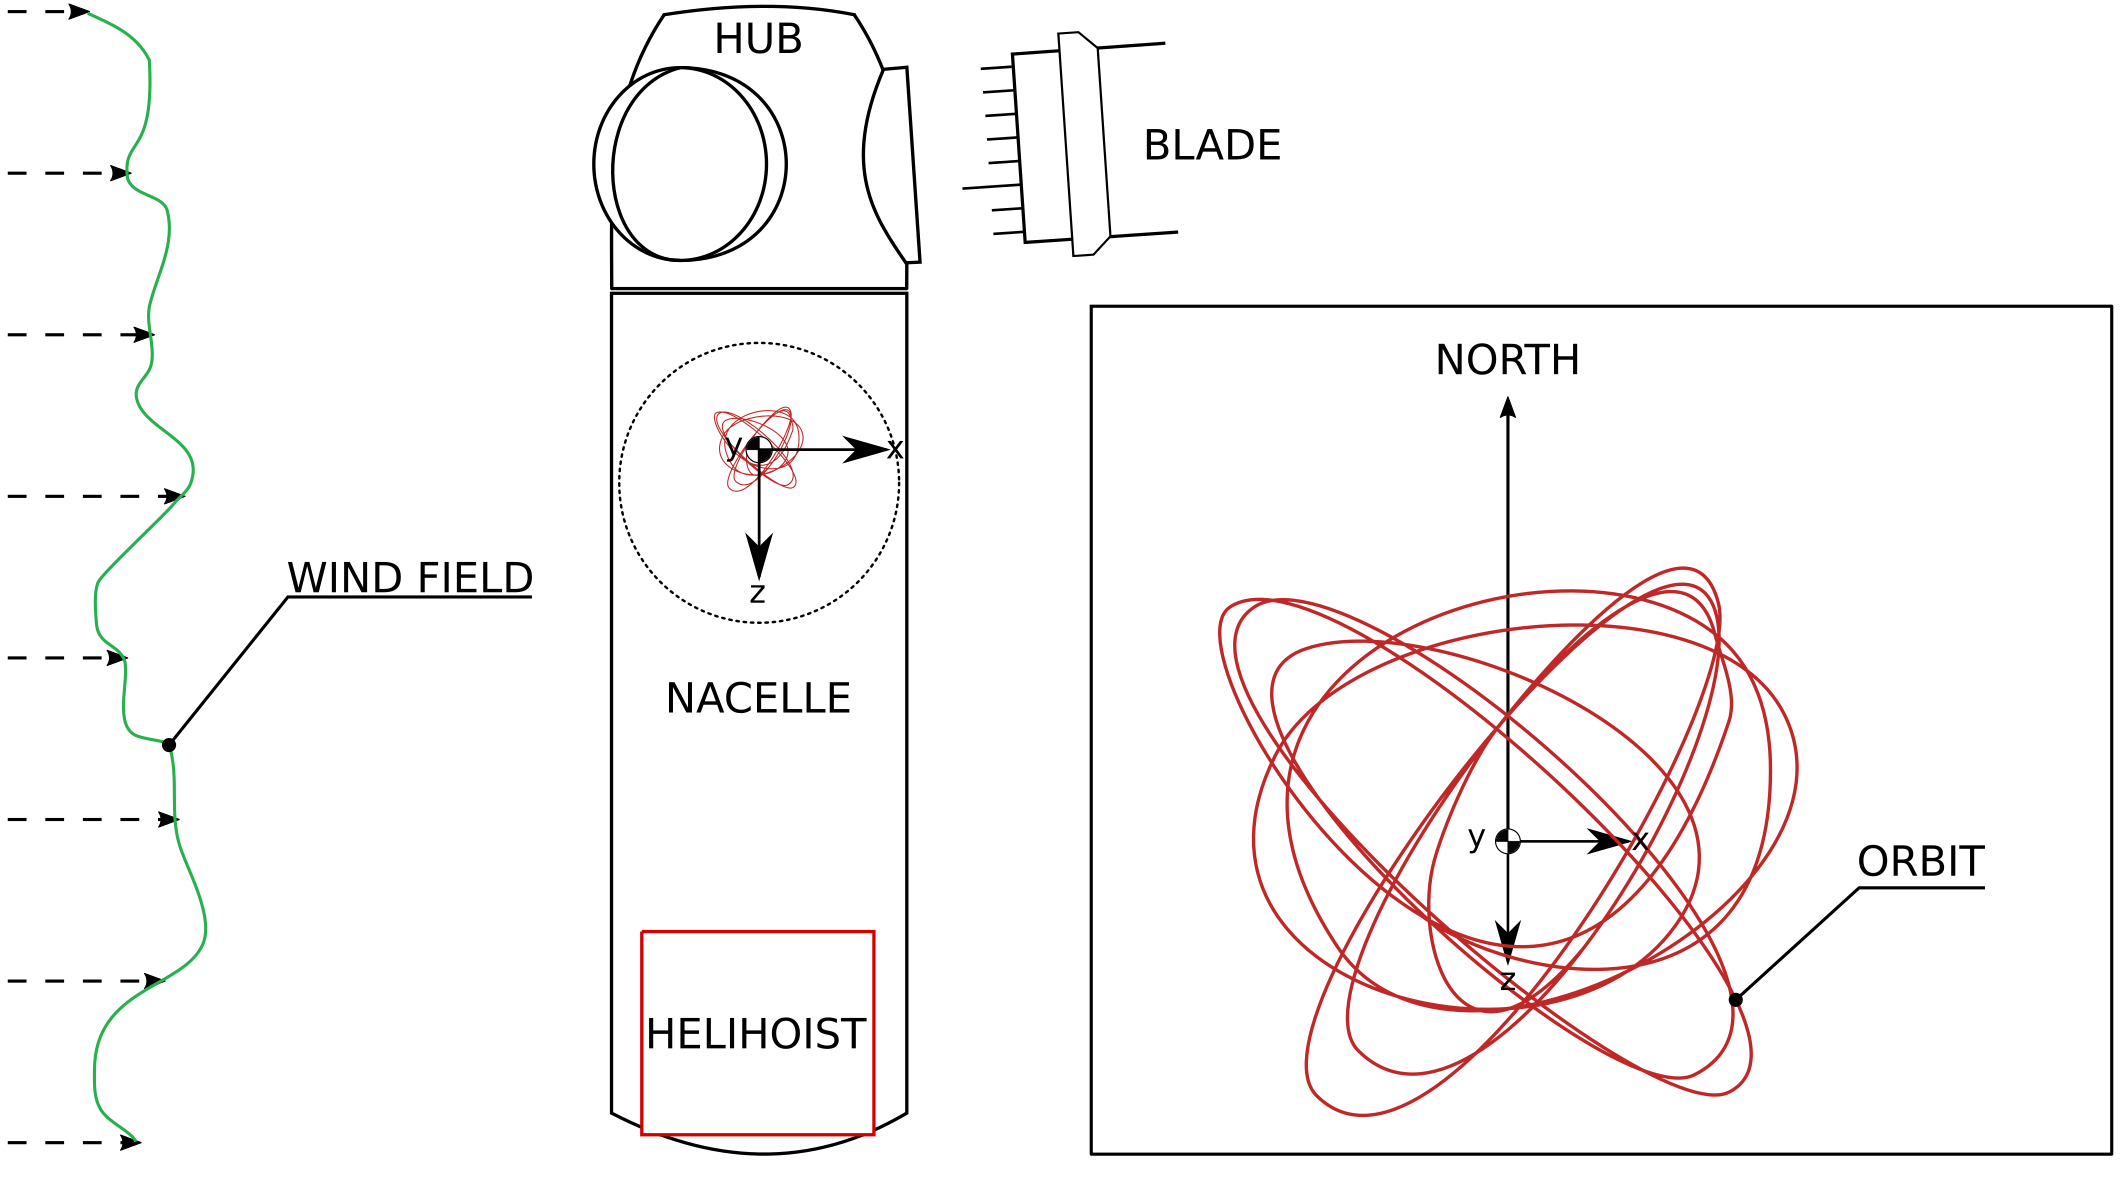
\includegraphics[width=0.7\linewidth]{figures/installation_alt2.png}
    \caption{Formation of orbits as observed during the installation of the offshore wind park \textit{Trianel Windpark Borkum II}. Note: the orbits are not to scale to enhance visibility.}
    \label{fig:orbit}
\end{figure}

Several mechanisms may in theory explain the formation of orbits. In this paper, we present a coupling mechanism that intrinsically leads to the formation of orbits in a cantilevered beam with an eccentric mass present. 

We focus on one specific state of an offshore wind turbine during installation: the hammerhead configuration. In this configuration, the foundation, transition piece, tower, and nacelle have already been installed, and the next installation step would be the installation of the first blade. In this configuration, the turbine is top heavy and, due to the nacelle's and rotor's weight, also nose-heavy. In the case of the turbines installed at \textit{Trianel Windpark Borkum II}, the centre of gravity of the nacelle is approximately 0.3 m shifted towards the rotor with respect to the tower axis. \autoref{fig:loading} depicts the hammerhead configuration as well as the simplified mechanical system derived to investigate the behaviour of partially installed turbines during installation. 

\begin{figure}[ht!]
    \centering
    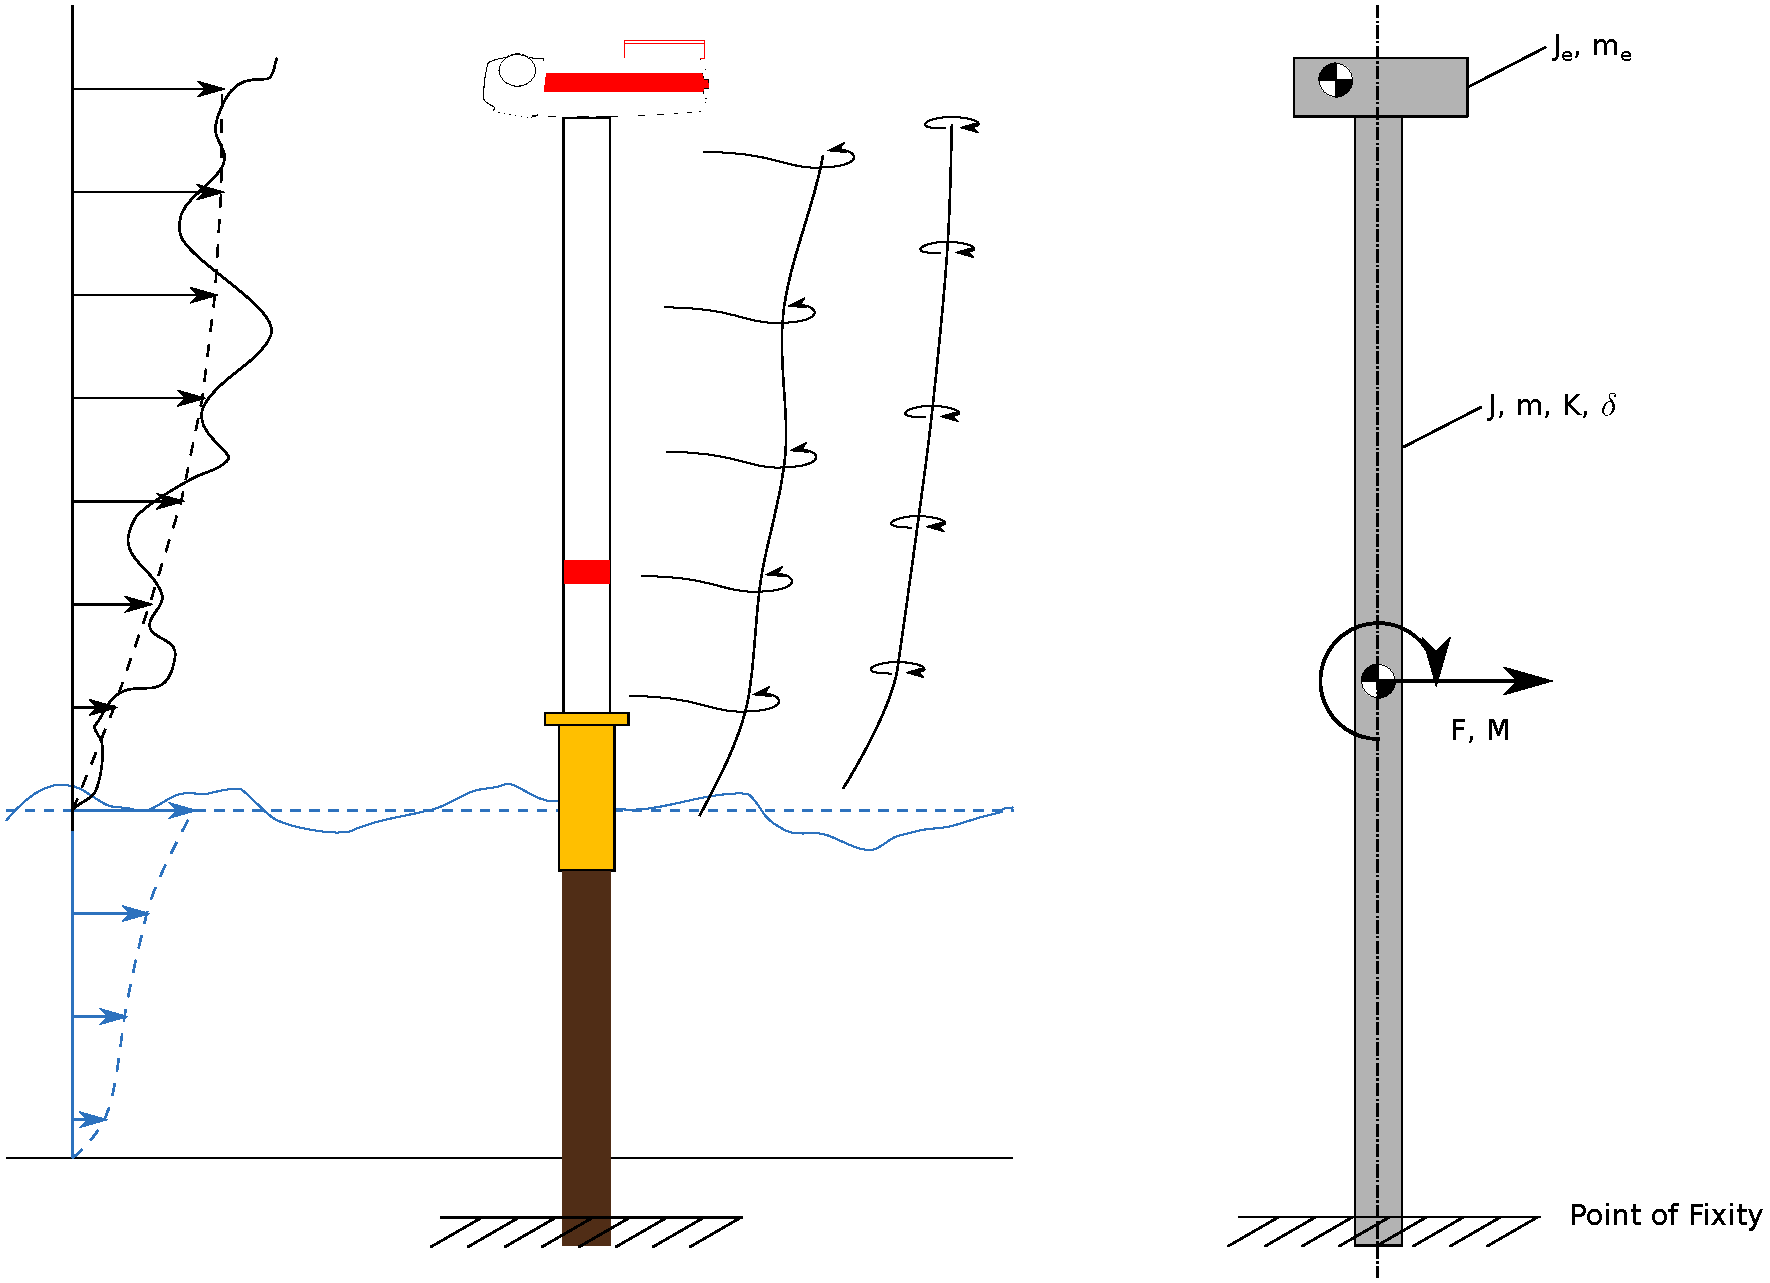
\includegraphics[width=0.7\linewidth]{figures/loading_3.pdf}
    \caption{Hammerhead configuration (left) and simplified mechanical model of the hammerhead configuration (right).}
    \label{fig:loading}
\end{figure}

The simplified system is a cantilevered beam with an eccentric mass at the free end. We hypothesize that the inertia of the eccentric mass leads to torsion of the cantilevered beam if the tower vibrates transversally. Twisting the tower along its main axis has two effects: a) the circular motion of the eccentric mass has a component perpendicular to the initial direction of motion, and thus momentum from that circular motion transfers into the perpendicular direction. b) twisting the tower leads to a torsional oscillation of the eccentric mass around the tower axis. The torsional motion of the eccentric mass in illustrated in \autoref{fig:kinematics}.

\clearpage

\begin{figure}[ht!]
    \centering
    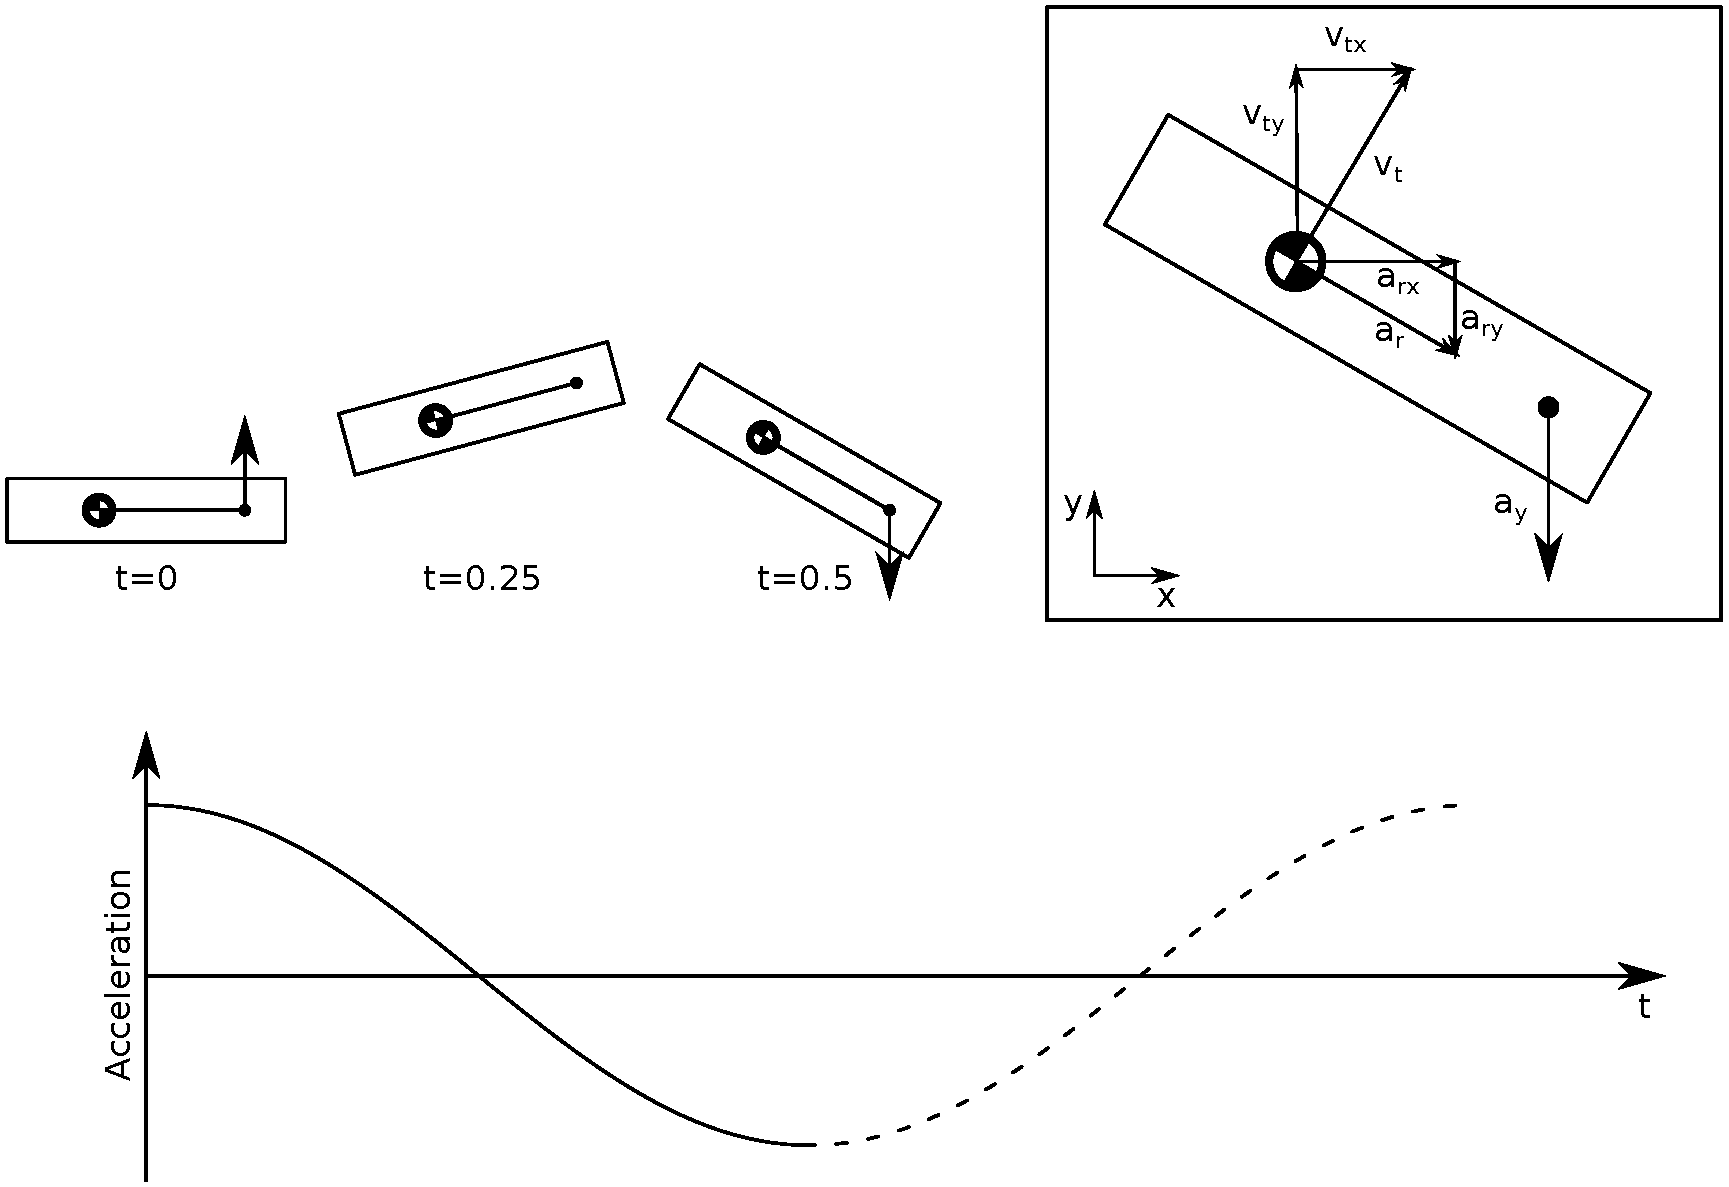
\includegraphics[width=0.7\linewidth]{figures/kinematics.pdf}
    \caption{Simplified kinematics of an eccentric mass undergoing harmonic oscillations.}
    \label{fig:kinematics}
\end{figure}

The paper is subdivided into four sections: first, results from a table-top experiment (\autoref{sec:experiment}), capable of reproducing the torsional coupling, are shown. A section on finite-element-simulations (\autoref{sec:simulations}) of a comparable system follows. Finally, a discrete system of differential equations (\autoref{sec:3dof}) is presented. The final section (\autoref{sec:discussion}) discusses the effect and the shortcomings of the presented approaches and discusses implications for future research into the topic. 

\clearpage

\section{Cantilever experiment}
\label{sec:experiment}

\subsection{Experimental Setup}

As a first proof of concept, we built a table-top experiment that allows us to demonstrate the effect of an eccentric mass on the vibration of a cantilevered beam. As a beam, we chose a wooden rod (massive beech, 0.006 m diameter) with a free length of 0.7 m. At the free end of the rod, we placed a 3D-printed lever that allowed us to add M8 bolts (0.028 m length, 0.0129 kg) to control the amount of eccentric mass. Lever length was 0.082 m weighing a total of 0.026 kg. A second rod made of fibre glass (diameter 0.008 m) was placed next to the cantilevered beam. \autoref{fig:setup} shows the experimental setup. The second rod was used to displace the cantilevered beam from its resting position  by pulling the cantilevered beam towards the second rod using a thin cotton thread. The initial displacement of the top of the rod was 0.135 m and three different masses (no bolts, two bolts, four bolts) were tested in the experiment. To release the cantilevered beam from it initial, displaced position, the thread was set on fire using a lighter. While this release mechanism seems somewhat archaic, it ensures that no external torque is added to the system upon release. For each mass, the experiment was repeated three times. A MEMS-based inertial measurement unit (MPU 9255, InvenSense TDK, Tokyo, Japan) placed on top of the cantilevered beam measured linear acceleration and angular velocity with a sampling rate of 100 Hz. Measurements were recorded using a Raspberry Pi 400 and a jupyter notebook with python3. All data and the corresponding code is available on github: \url{https://github.com/k323r/2021_preprint_eccentric-mass}.

\begin{figure}[ht!]
    \centering
    \includegraphics[width=0.5\linewidth]{figures/setup.png}
    \caption{Experimental setup}
    \label{fig:setup}
\end{figure}

The following post-processing steps have been applied to the recorded data:

First, obtained accelerations in fore-aft and side-side direction were resampled to 50 Hz using linear interpolation. 

As the data is indexed by the time of the recording, the time series of each experiment had to be normalized to enable comparison of the different time series. The first peak in the fore-aft acceleration signal in each recorded experiment served as a normalization time stamp; Each signal was cropped, such that it starts 0.5 s prior to the first peak and lasts for 120 s. 

Following time normalization, the data was filtered by applying a Butterworth high-pass filter with a cut-off frequency of 0.5 Hz, order 11 and padding of 25 s to remove any transient effects. The filter was applied forwards and backwards in time to remove any frequency response (phase delay). Afterwards, the accelerations and the angular velocities were integrated using a second order trapeze type integration, yielding the velocity vector of the rod's tip and the torsion angle of the rod. To obtain the displacement vector, the velocity vector was filtered again with the same Butterworth filter, integrated again and finally both torsion angle and displacement vector were filtered one last time with the same Butterworth filter.

To compare experimental measurements with finite element simulations and the 3-DoF model (both without damping), the observed displacement from the experimental results was normalized to remove the influence of damping from the observed orbits. To this end, the observed decay in displacement amplitude over time is estimated using an exponential function of the following form:

\begin{equation}
    A = A_0 e ^ {\gamma t} + a
\end{equation}

where $A_0$ is the initial amplitude, $\gamma$ is the damping coefficient and $a$ is a constant offset to account for the finite time series. To obtain orbits free of damping, the displacement vector is scaled by the exponential decay function. 

\subsection{Experimental Results}

\autoref{fig:low-mass}, \autoref{fig:medium-mass} and \autoref{fig:high-mass} each show the observed accelerations, the angular velocity along the rod main axis and the absolute acceleration in the fore-aft-side-side plane as well as the corresponding orbits.

%%%
% Low mass
%%%

\begin{figure*}[ht]

    \centering
    \begin{subfigure}[b]{0.45\textwidth}
        \centering
        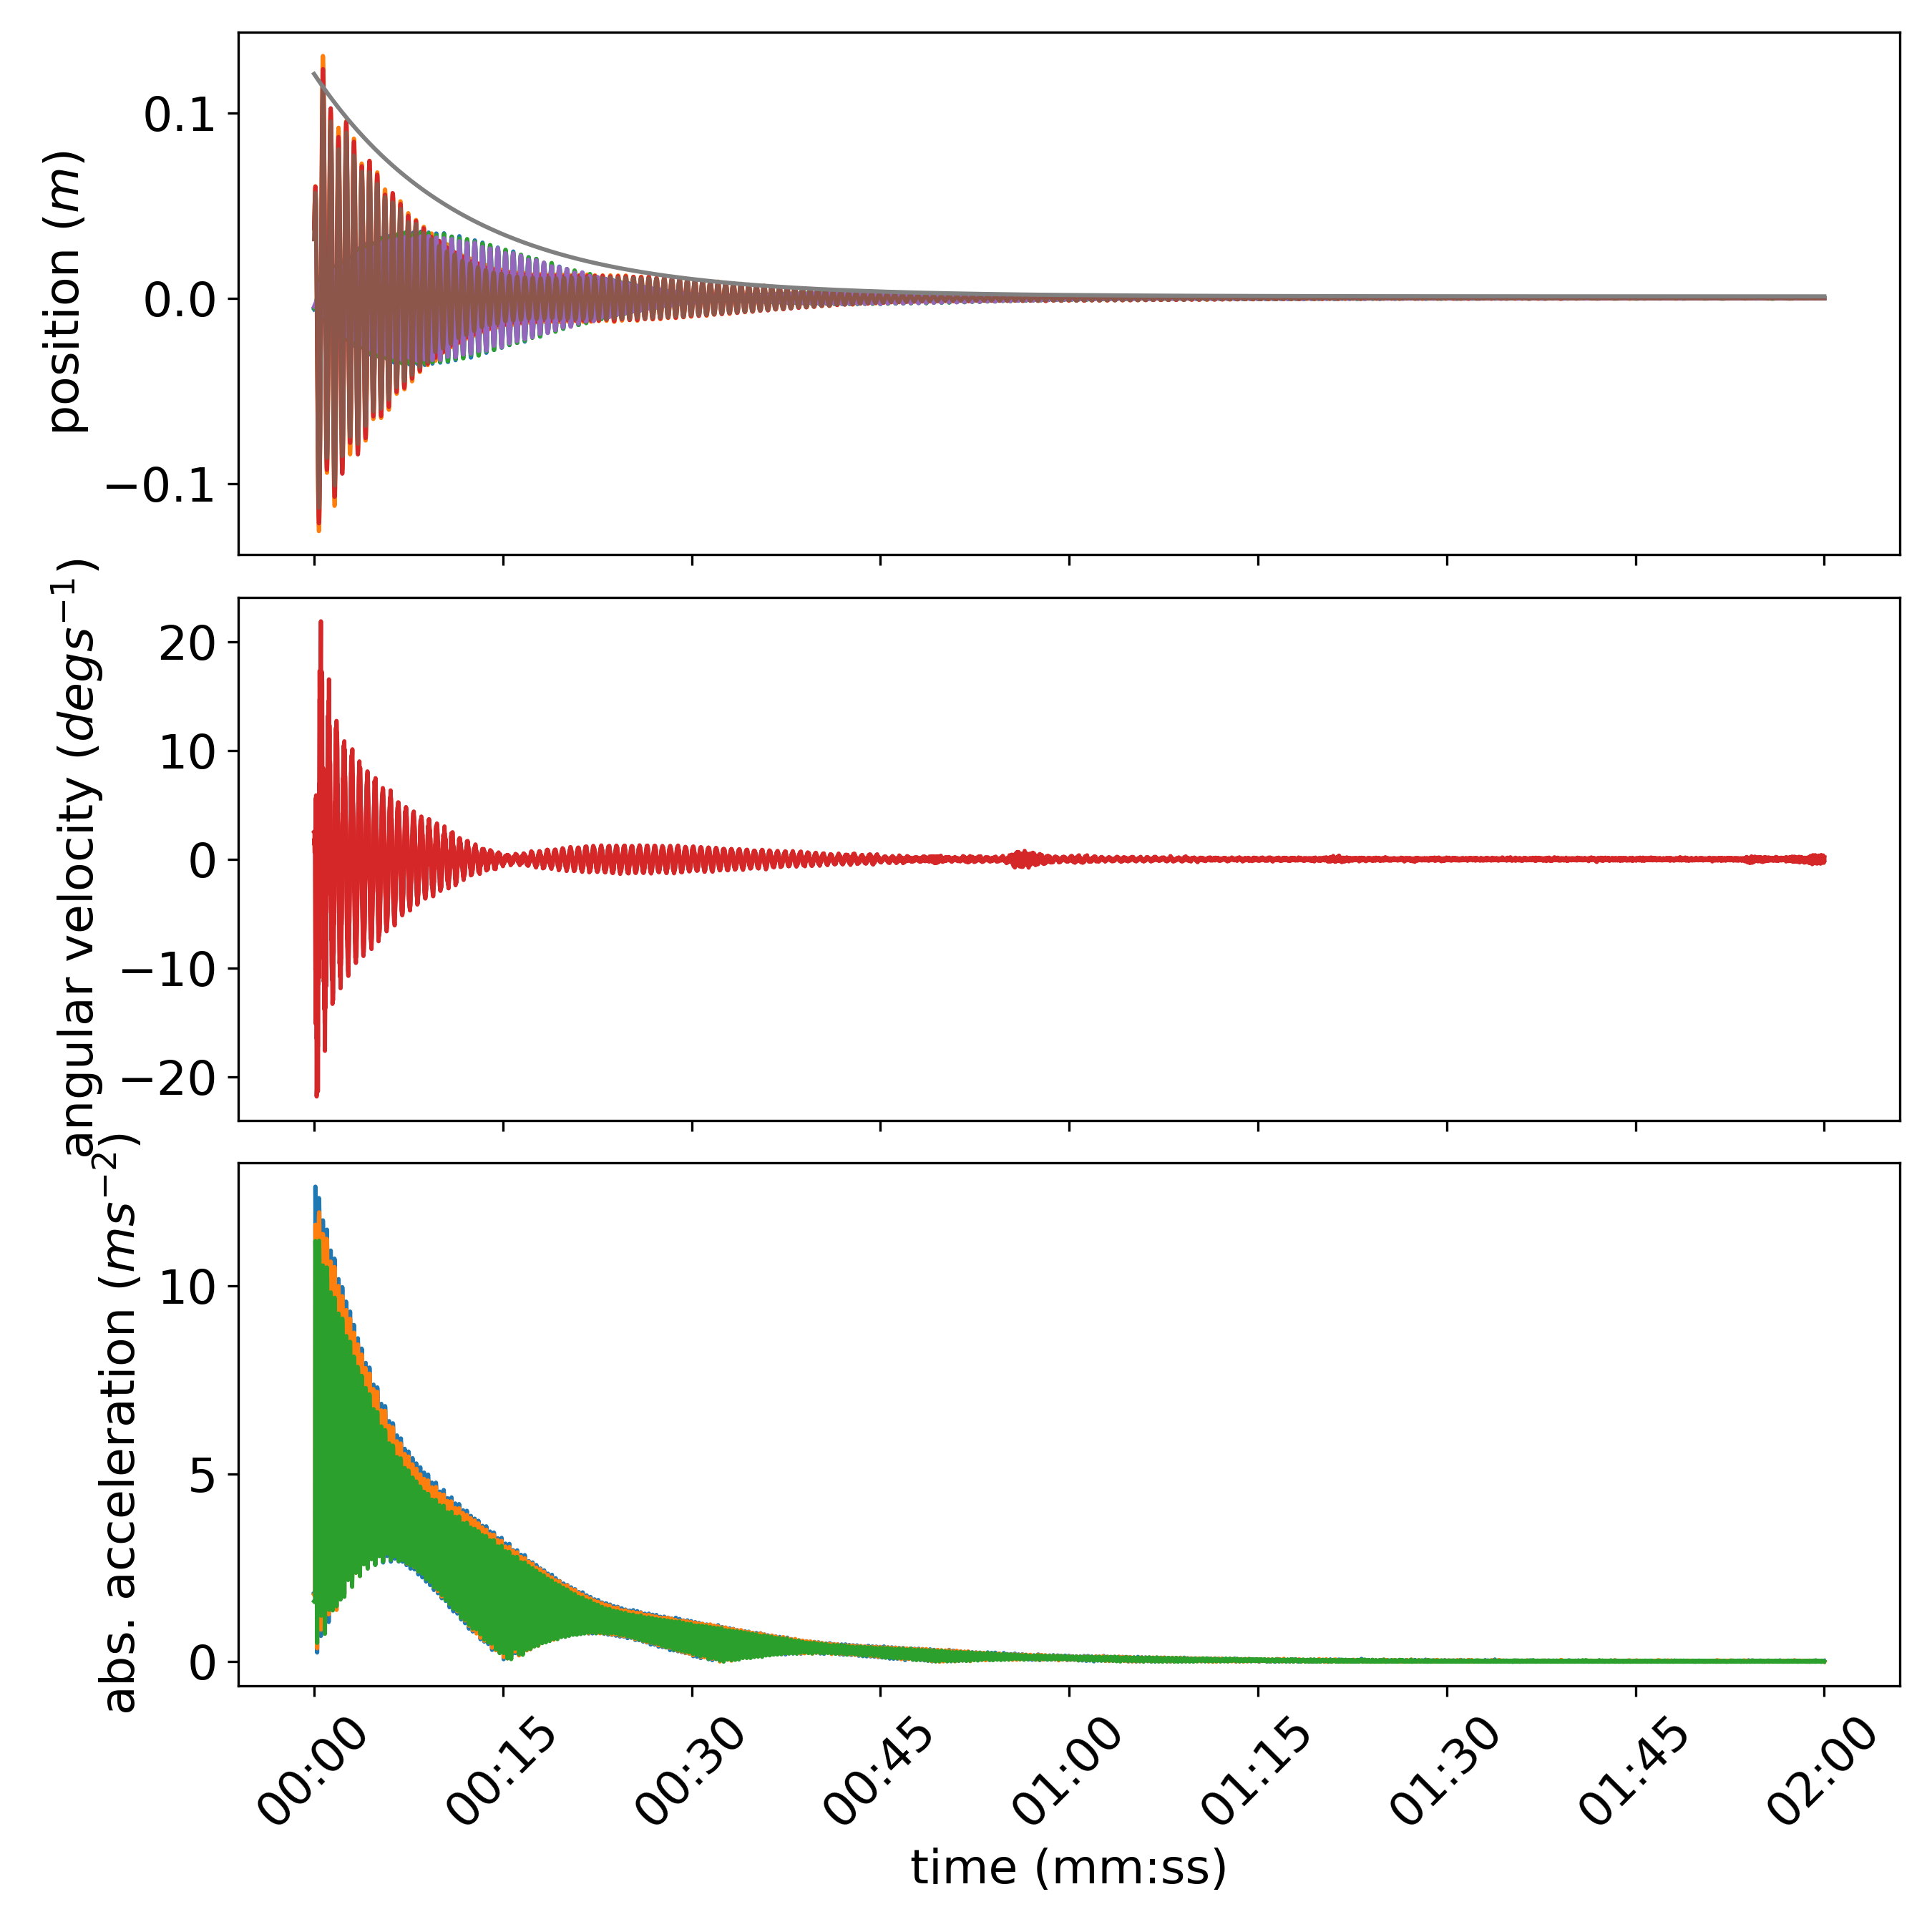
\includegraphics[width=\textwidth]{../results/experiment/low_mass_acceleration.png}
        \caption{}
        % \caption{Scatter diagram for mean deflection $d_{10}$ and significant wave height $H_{S10}$. The linear fit is shown as a blue line.}
        \label{fig:low-mass:acc}
    \end{subfigure}
    \begin{subfigure}[b]{0.45\textwidth}
        \centering
        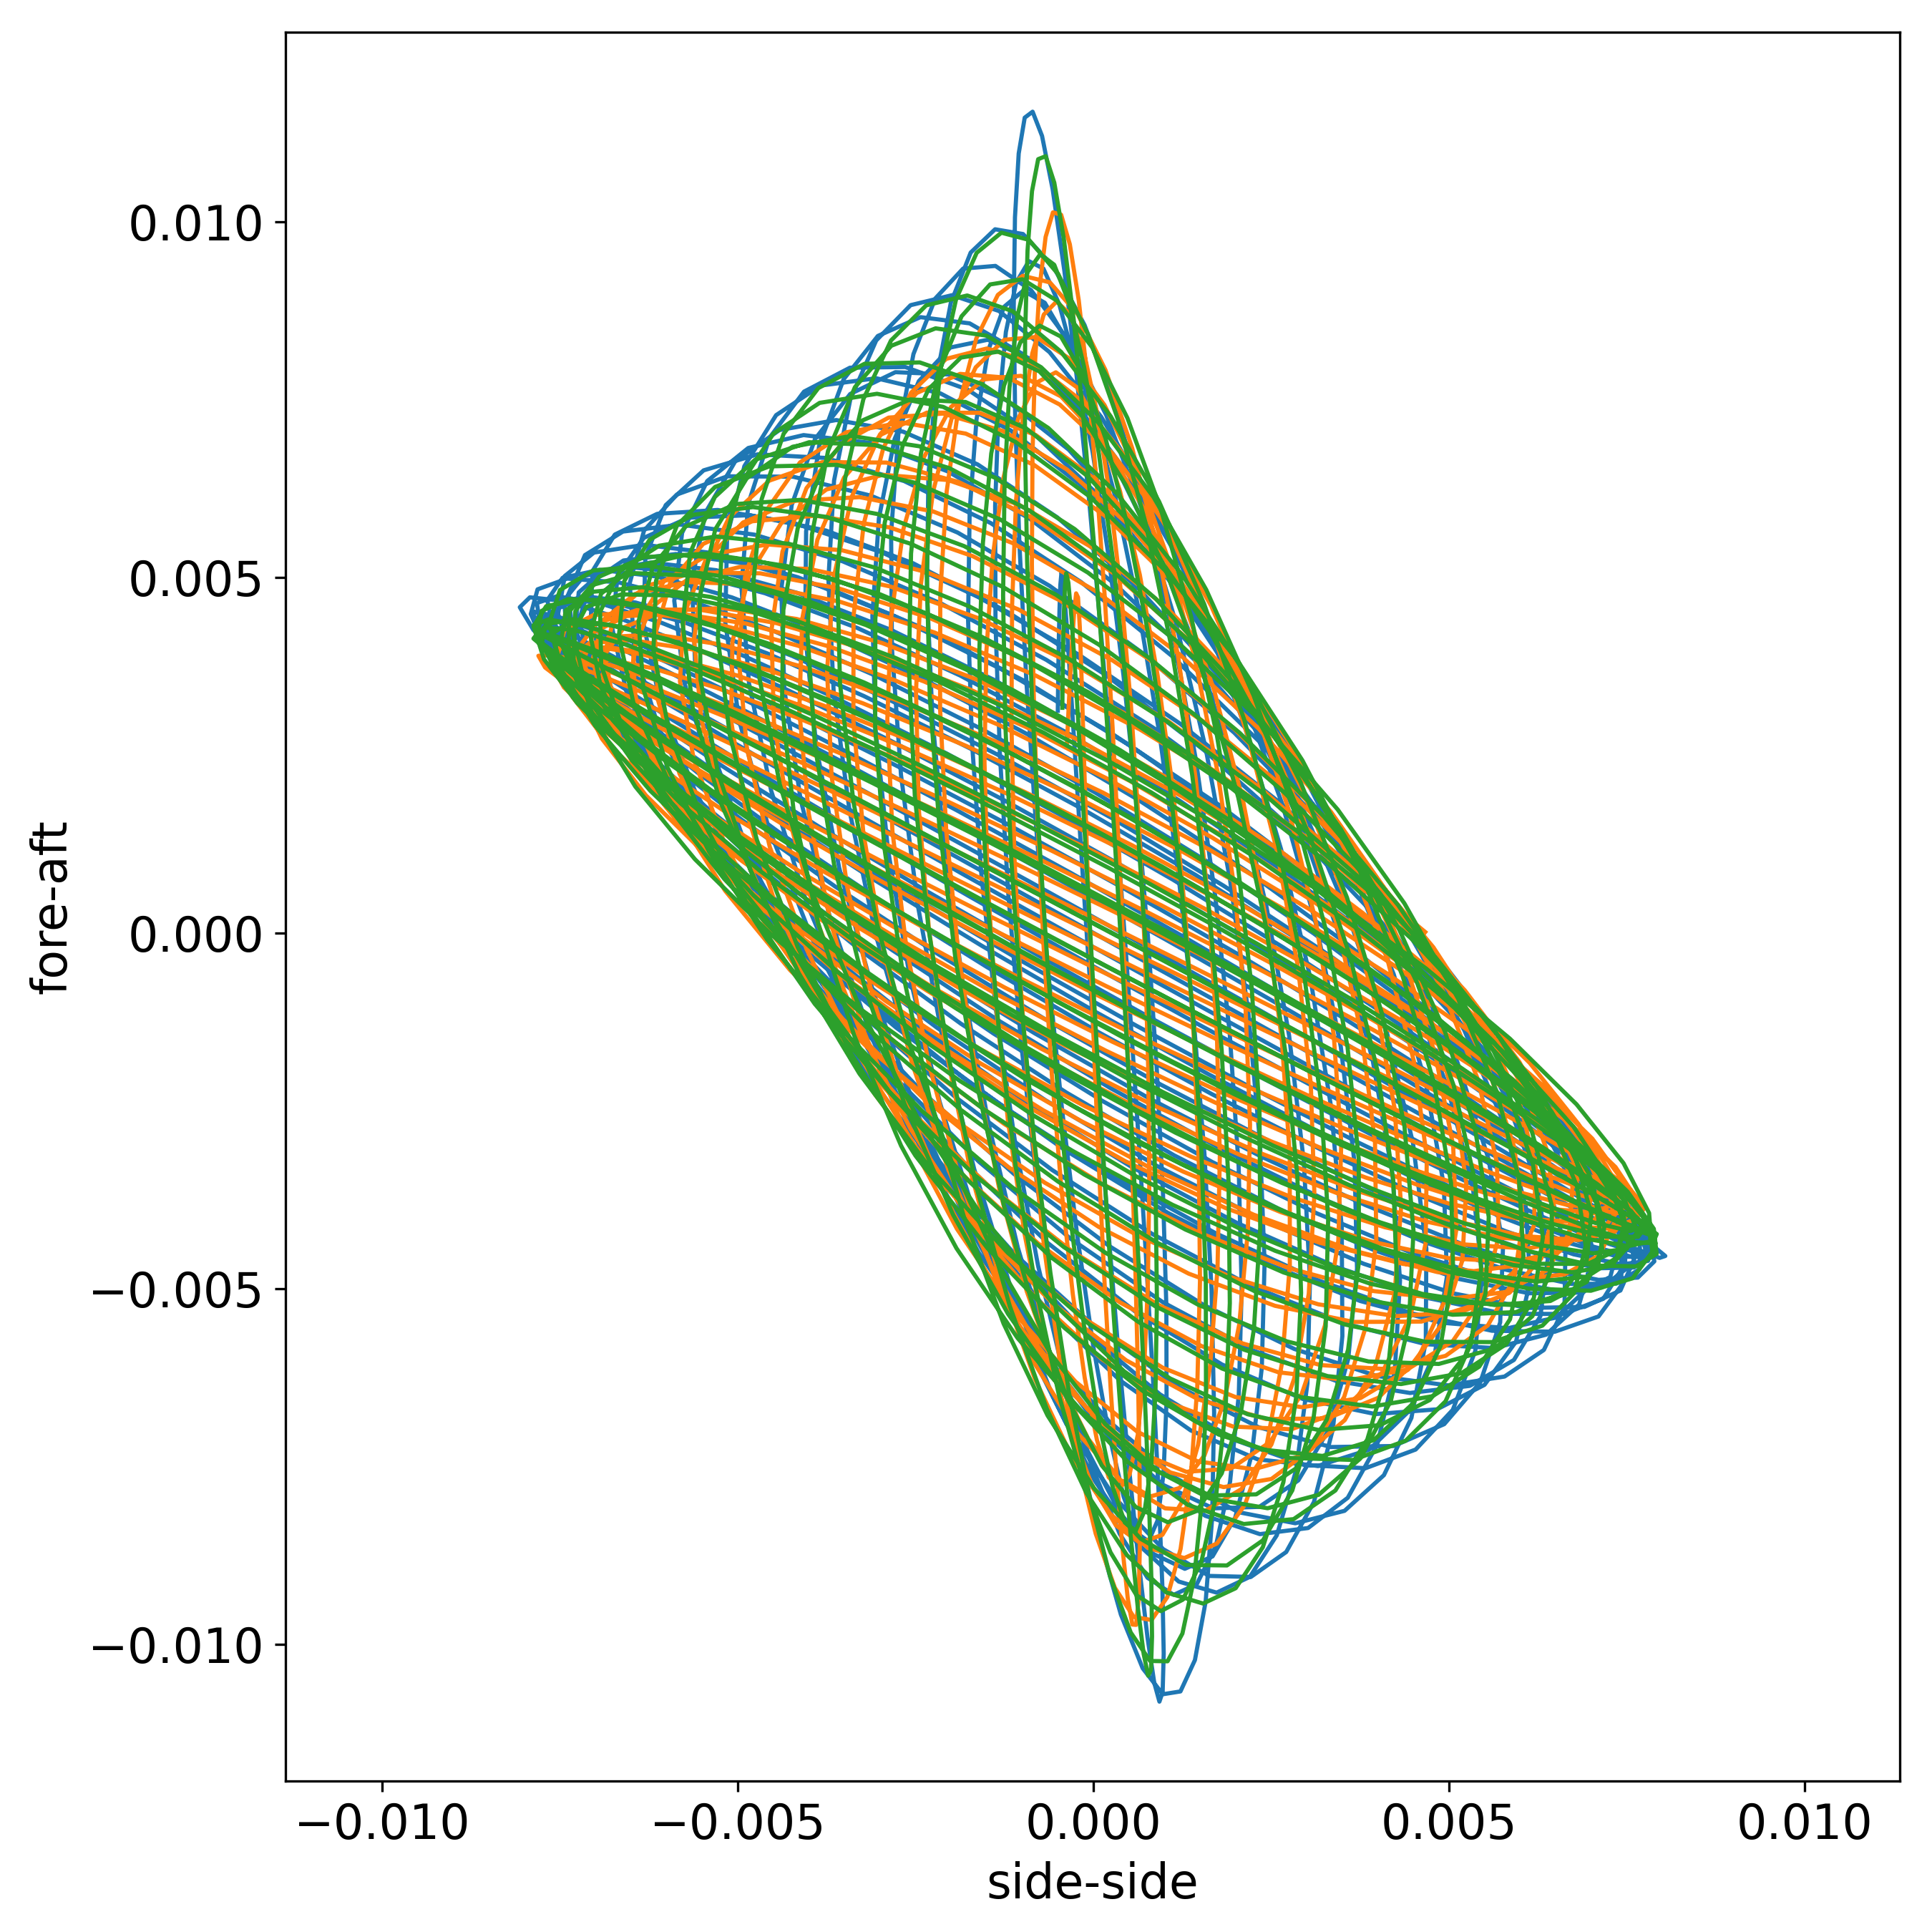
\includegraphics[width=\textwidth]{../results/experiment/low_mass_orbit.png}
        \caption{}
        % \caption{Scatter diagram for mean deflection $d_{10}$ and significant wave height $H_{S10}$. The linear fit is shown as a blue line.}
        \label{fig:low-mass:orbit}
    \end{subfigure}
    
    \caption{Accelerations, angular velocity and absolute acceleration (left) and Lissajous figures (orbits) for the low mass scenario.}
    \label{fig:low-mass}
\end{figure*}

%%%
% medium mass
%%%

\begin{figure*}

    \centering
    \begin{subfigure}[b]{0.45\textwidth}
        \centering
        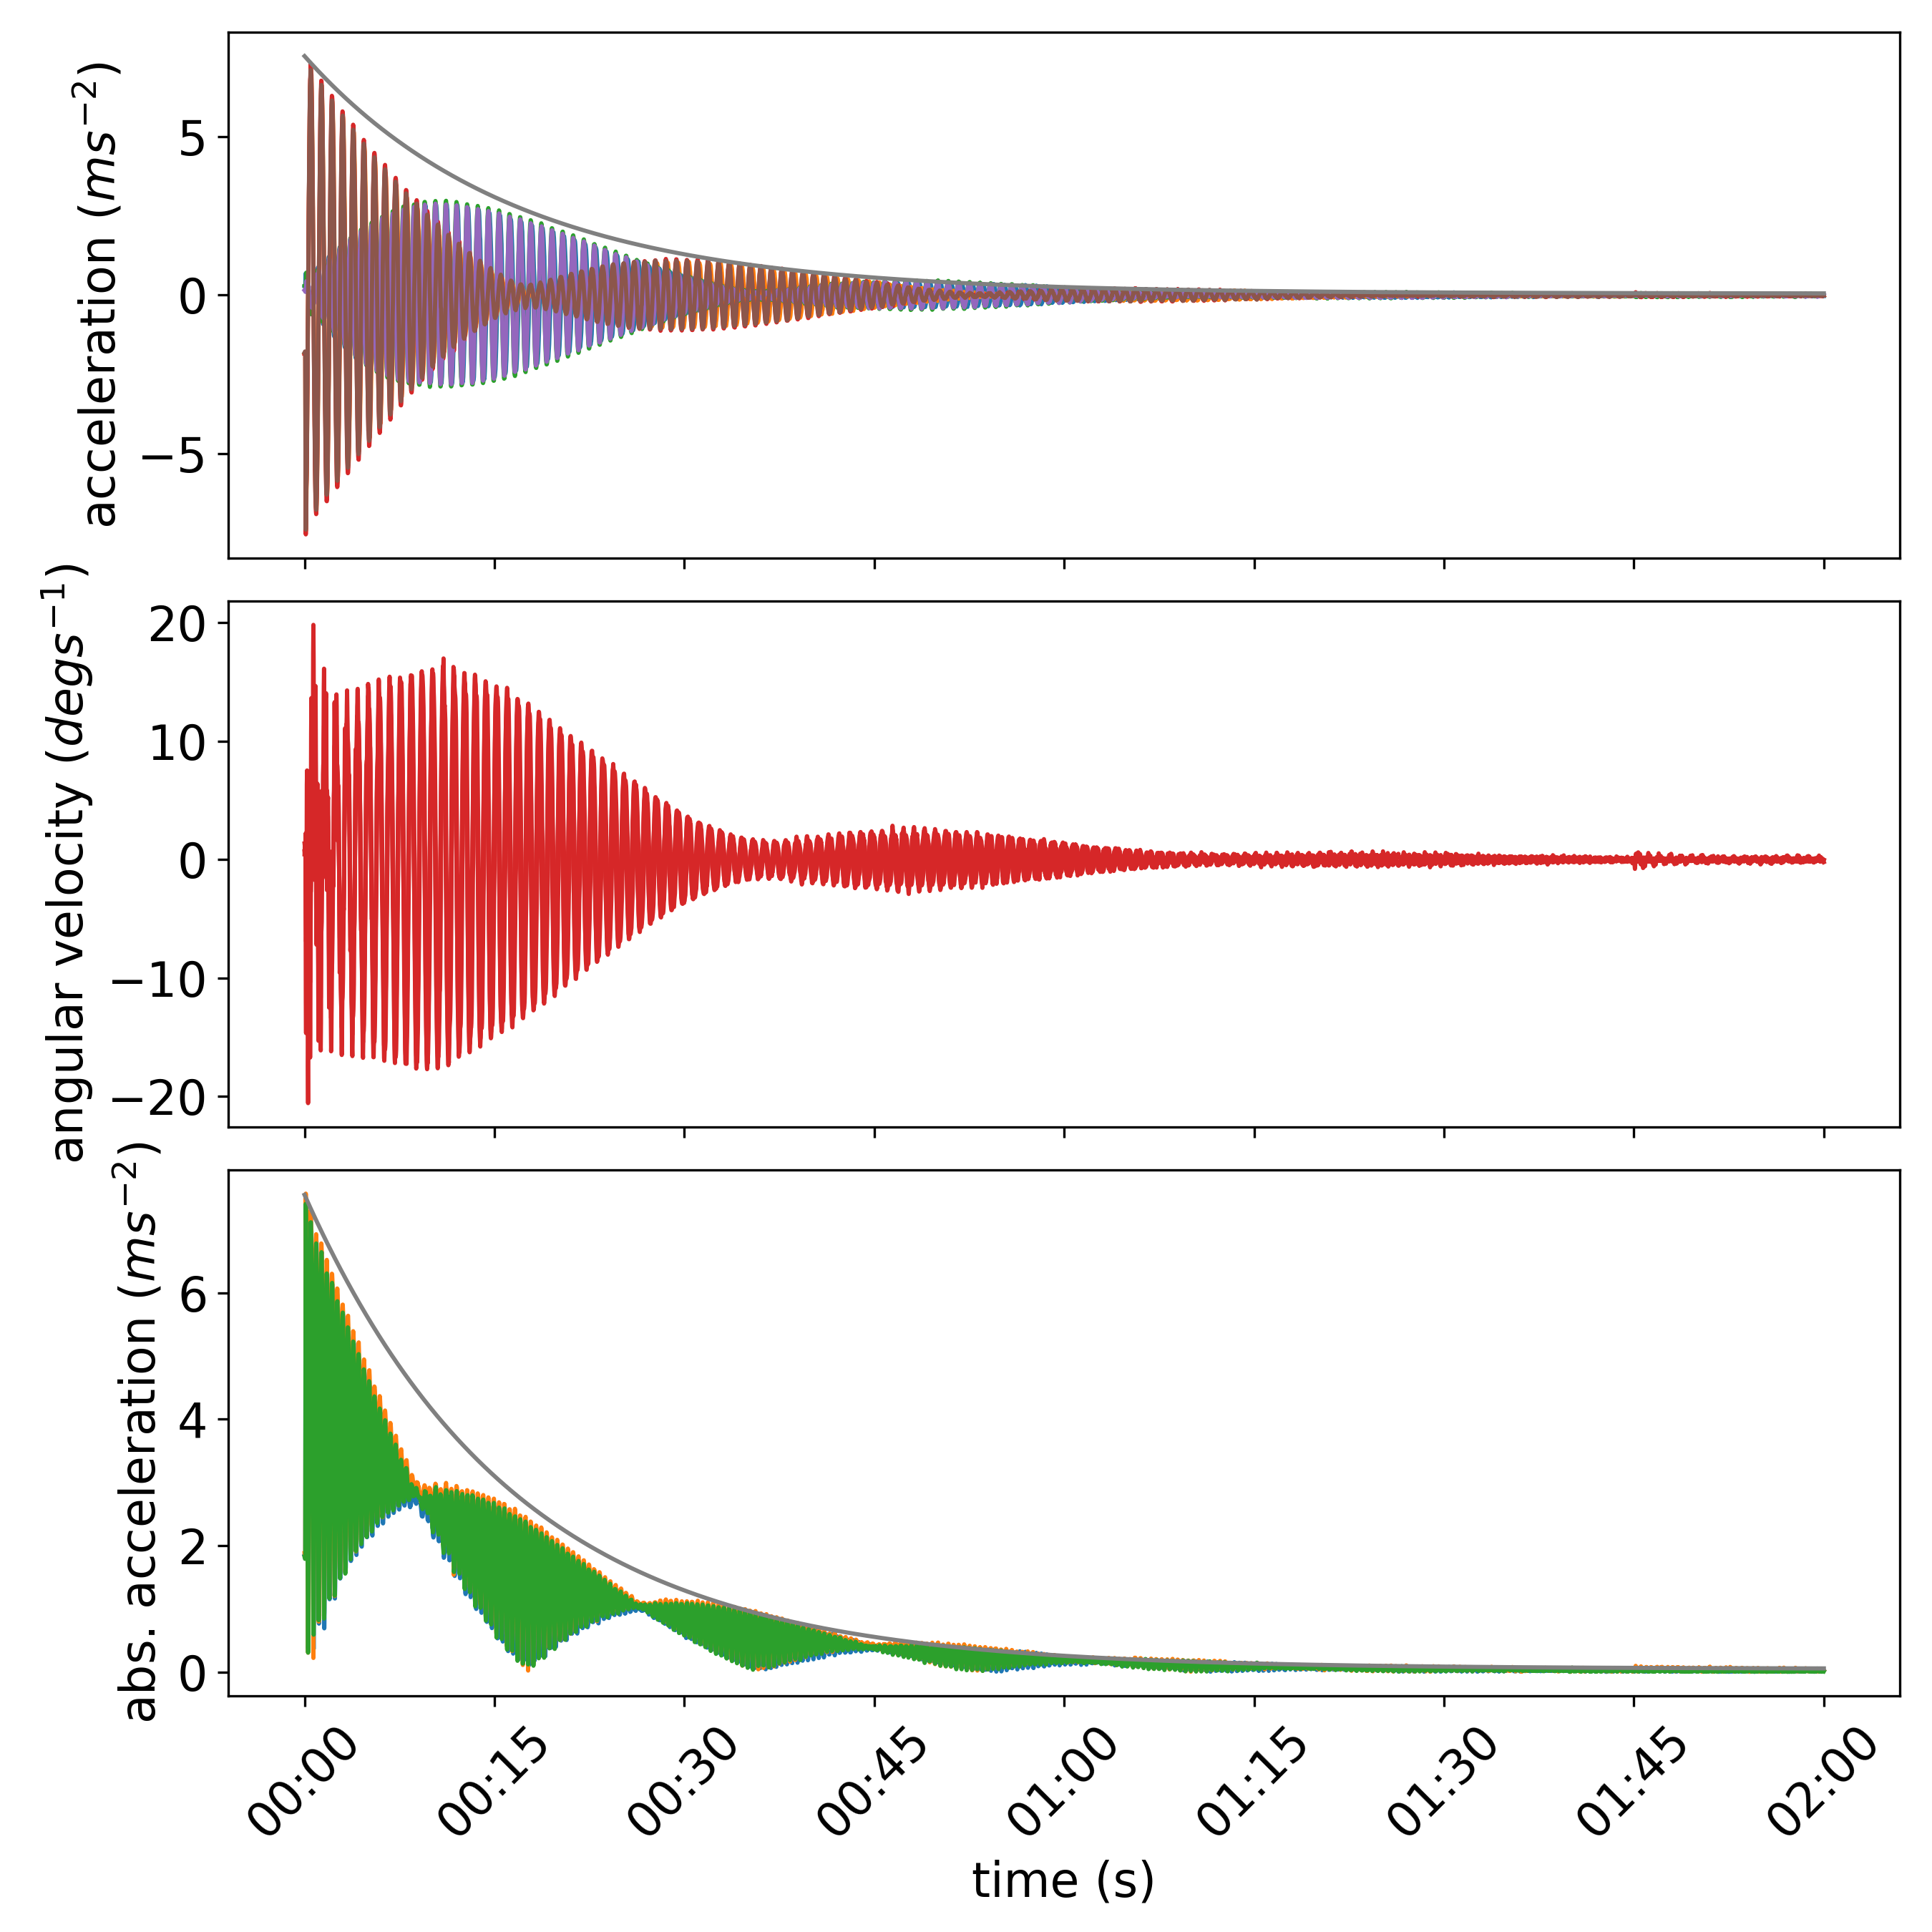
\includegraphics[width=\textwidth]{../results/experiment/medium_mass_acceleration.png}
        \caption{}
        % \caption{Scatter diagram for mean deflection $d_{10}$ and significant wave height $H_{S10}$. The linear fit is shown as a blue line.}
        \label{fig:medium-mass:acc}
    \end{subfigure}
    \begin{subfigure}[b]{0.45\textwidth}
        \centering
        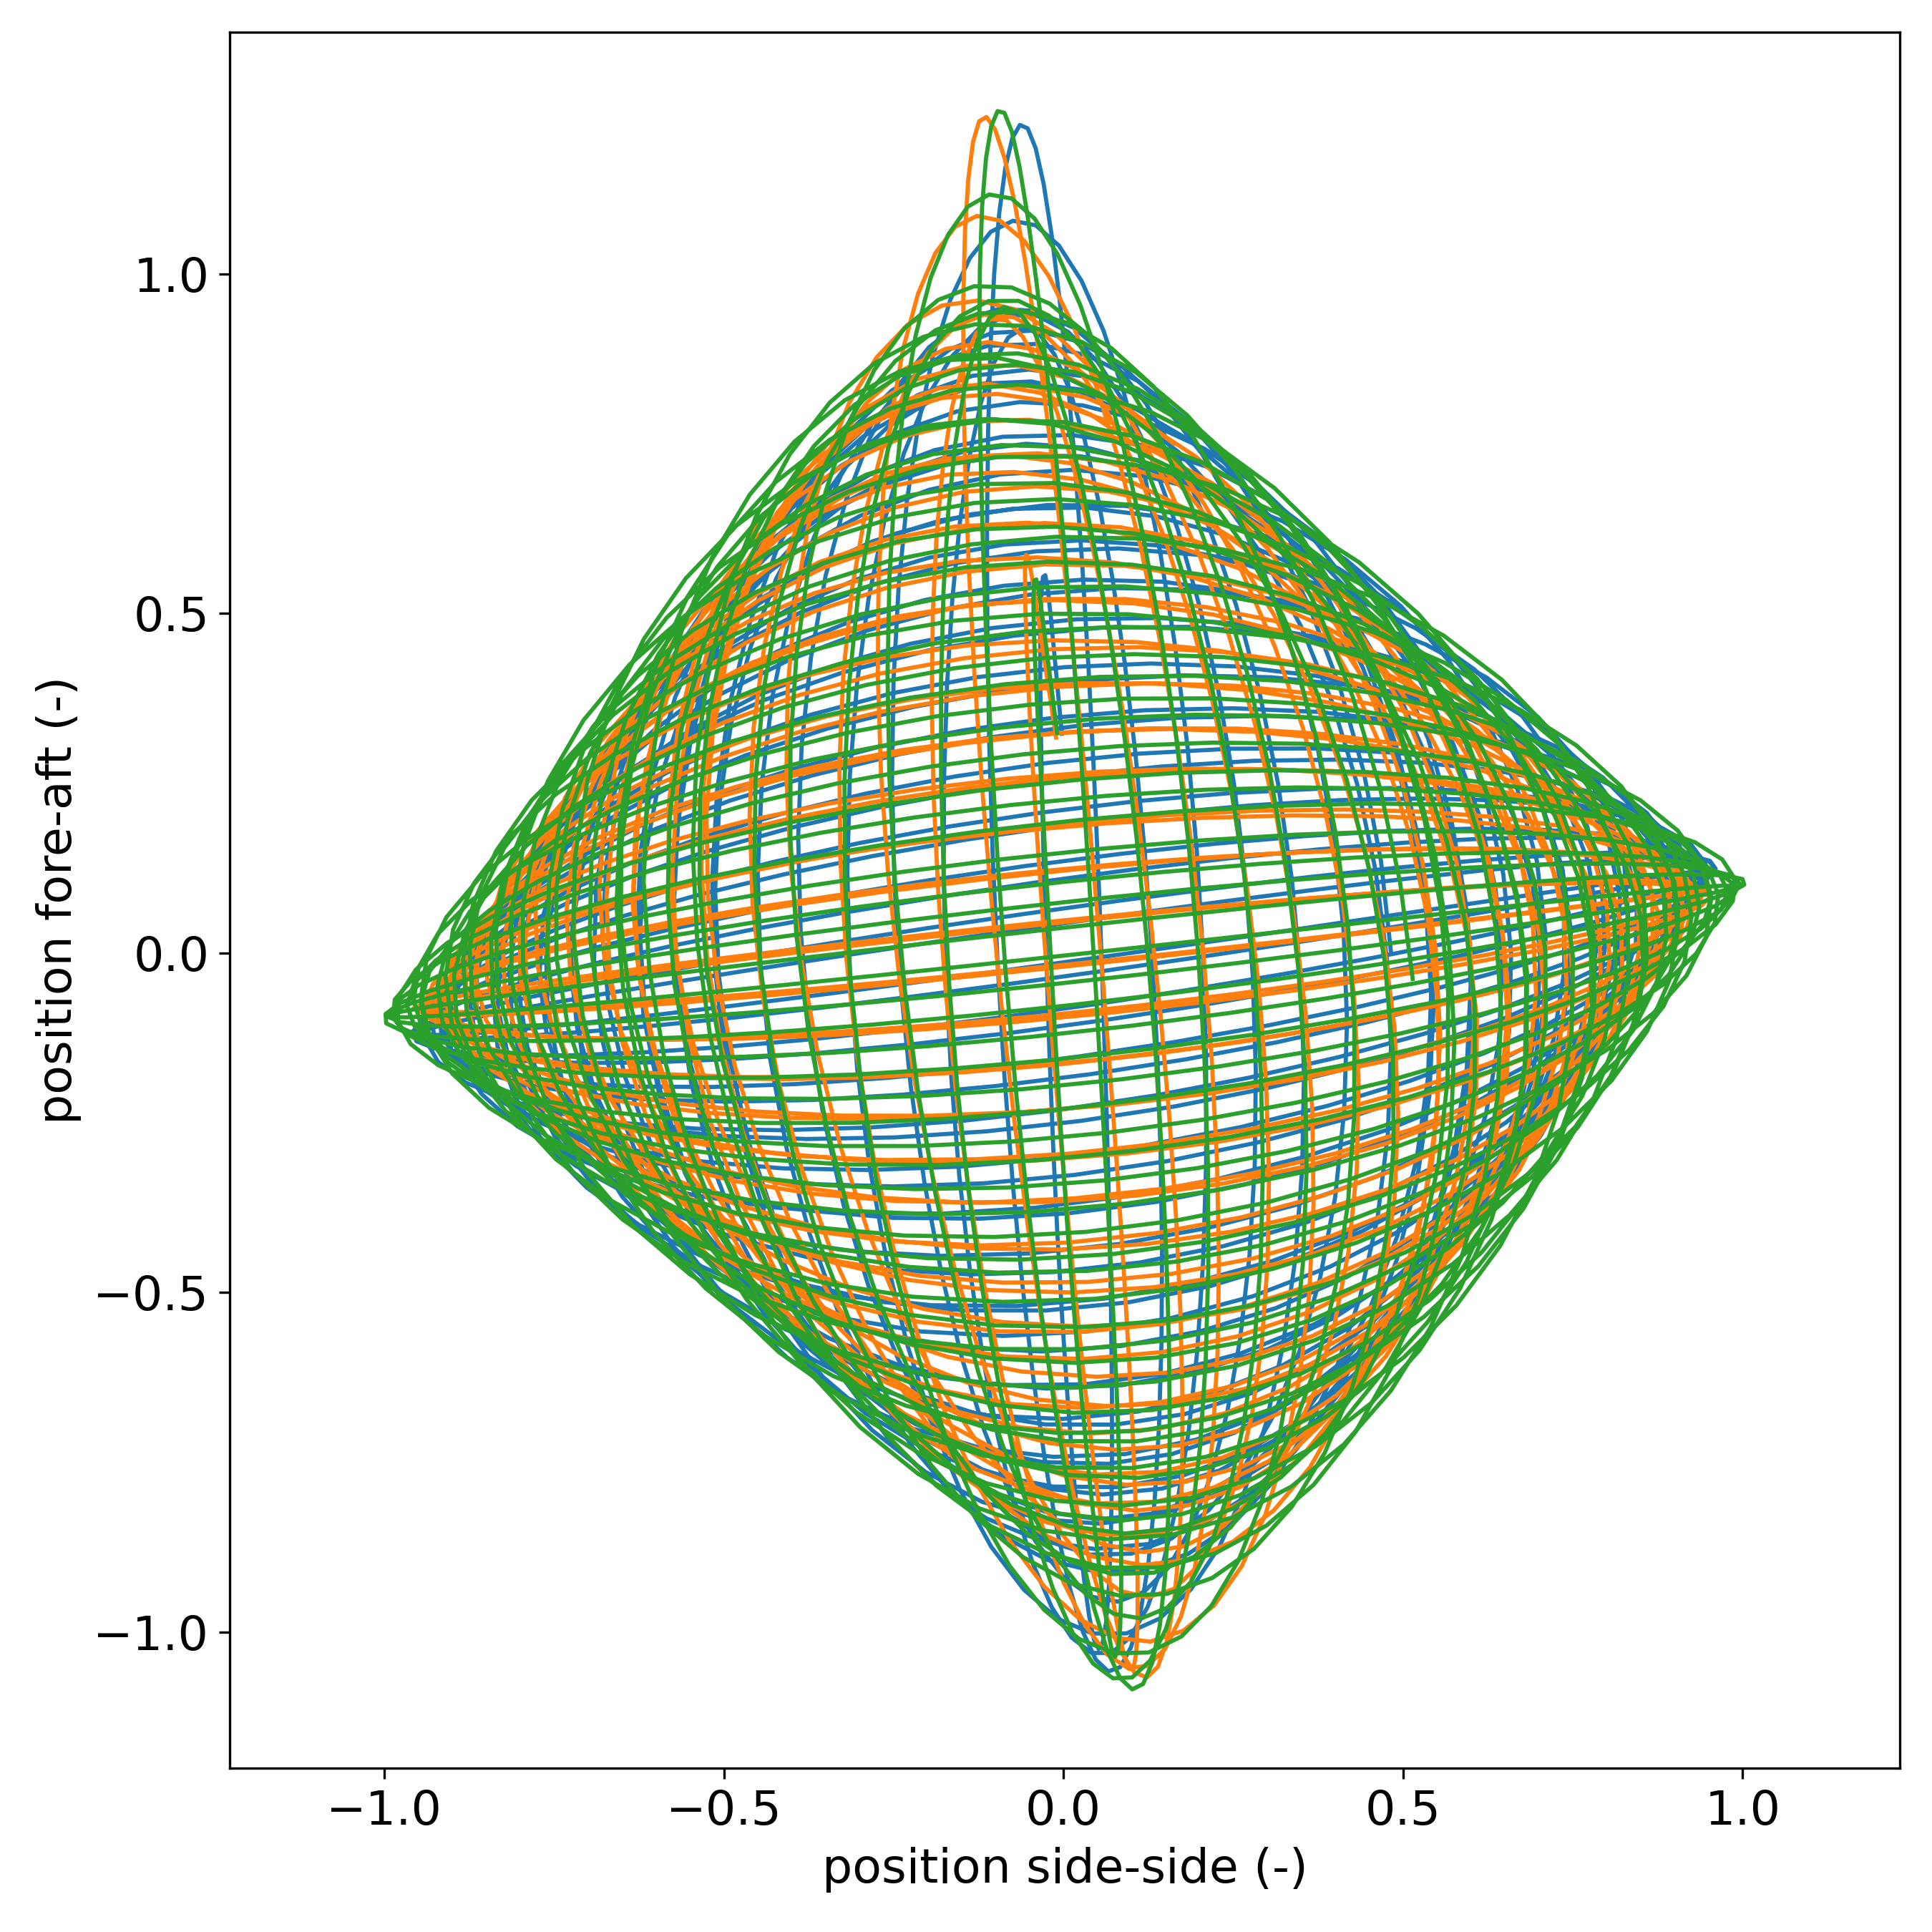
\includegraphics[width=\textwidth]{../results/experiment/medium_mass_orbit.png}
        \caption{}
        % \caption{Scatter diagram for mean deflection $d_{10}$ and significant wave height $H_{S10}$. The linear fit is shown as a blue line.}
        \label{fig:medium-mass:orbit}
    \end{subfigure}
    
    \caption{Accelerations, angular velocity and absolute acceleration (left) and Lissajous figures (orbits) for the medium mass scenario.}
    \label{fig:medium-mass}
\end{figure*}

%%%
% High mass
%%%

\begin{figure*}

    \centering
    \begin{subfigure}[b]{0.45\textwidth}
        \centering
        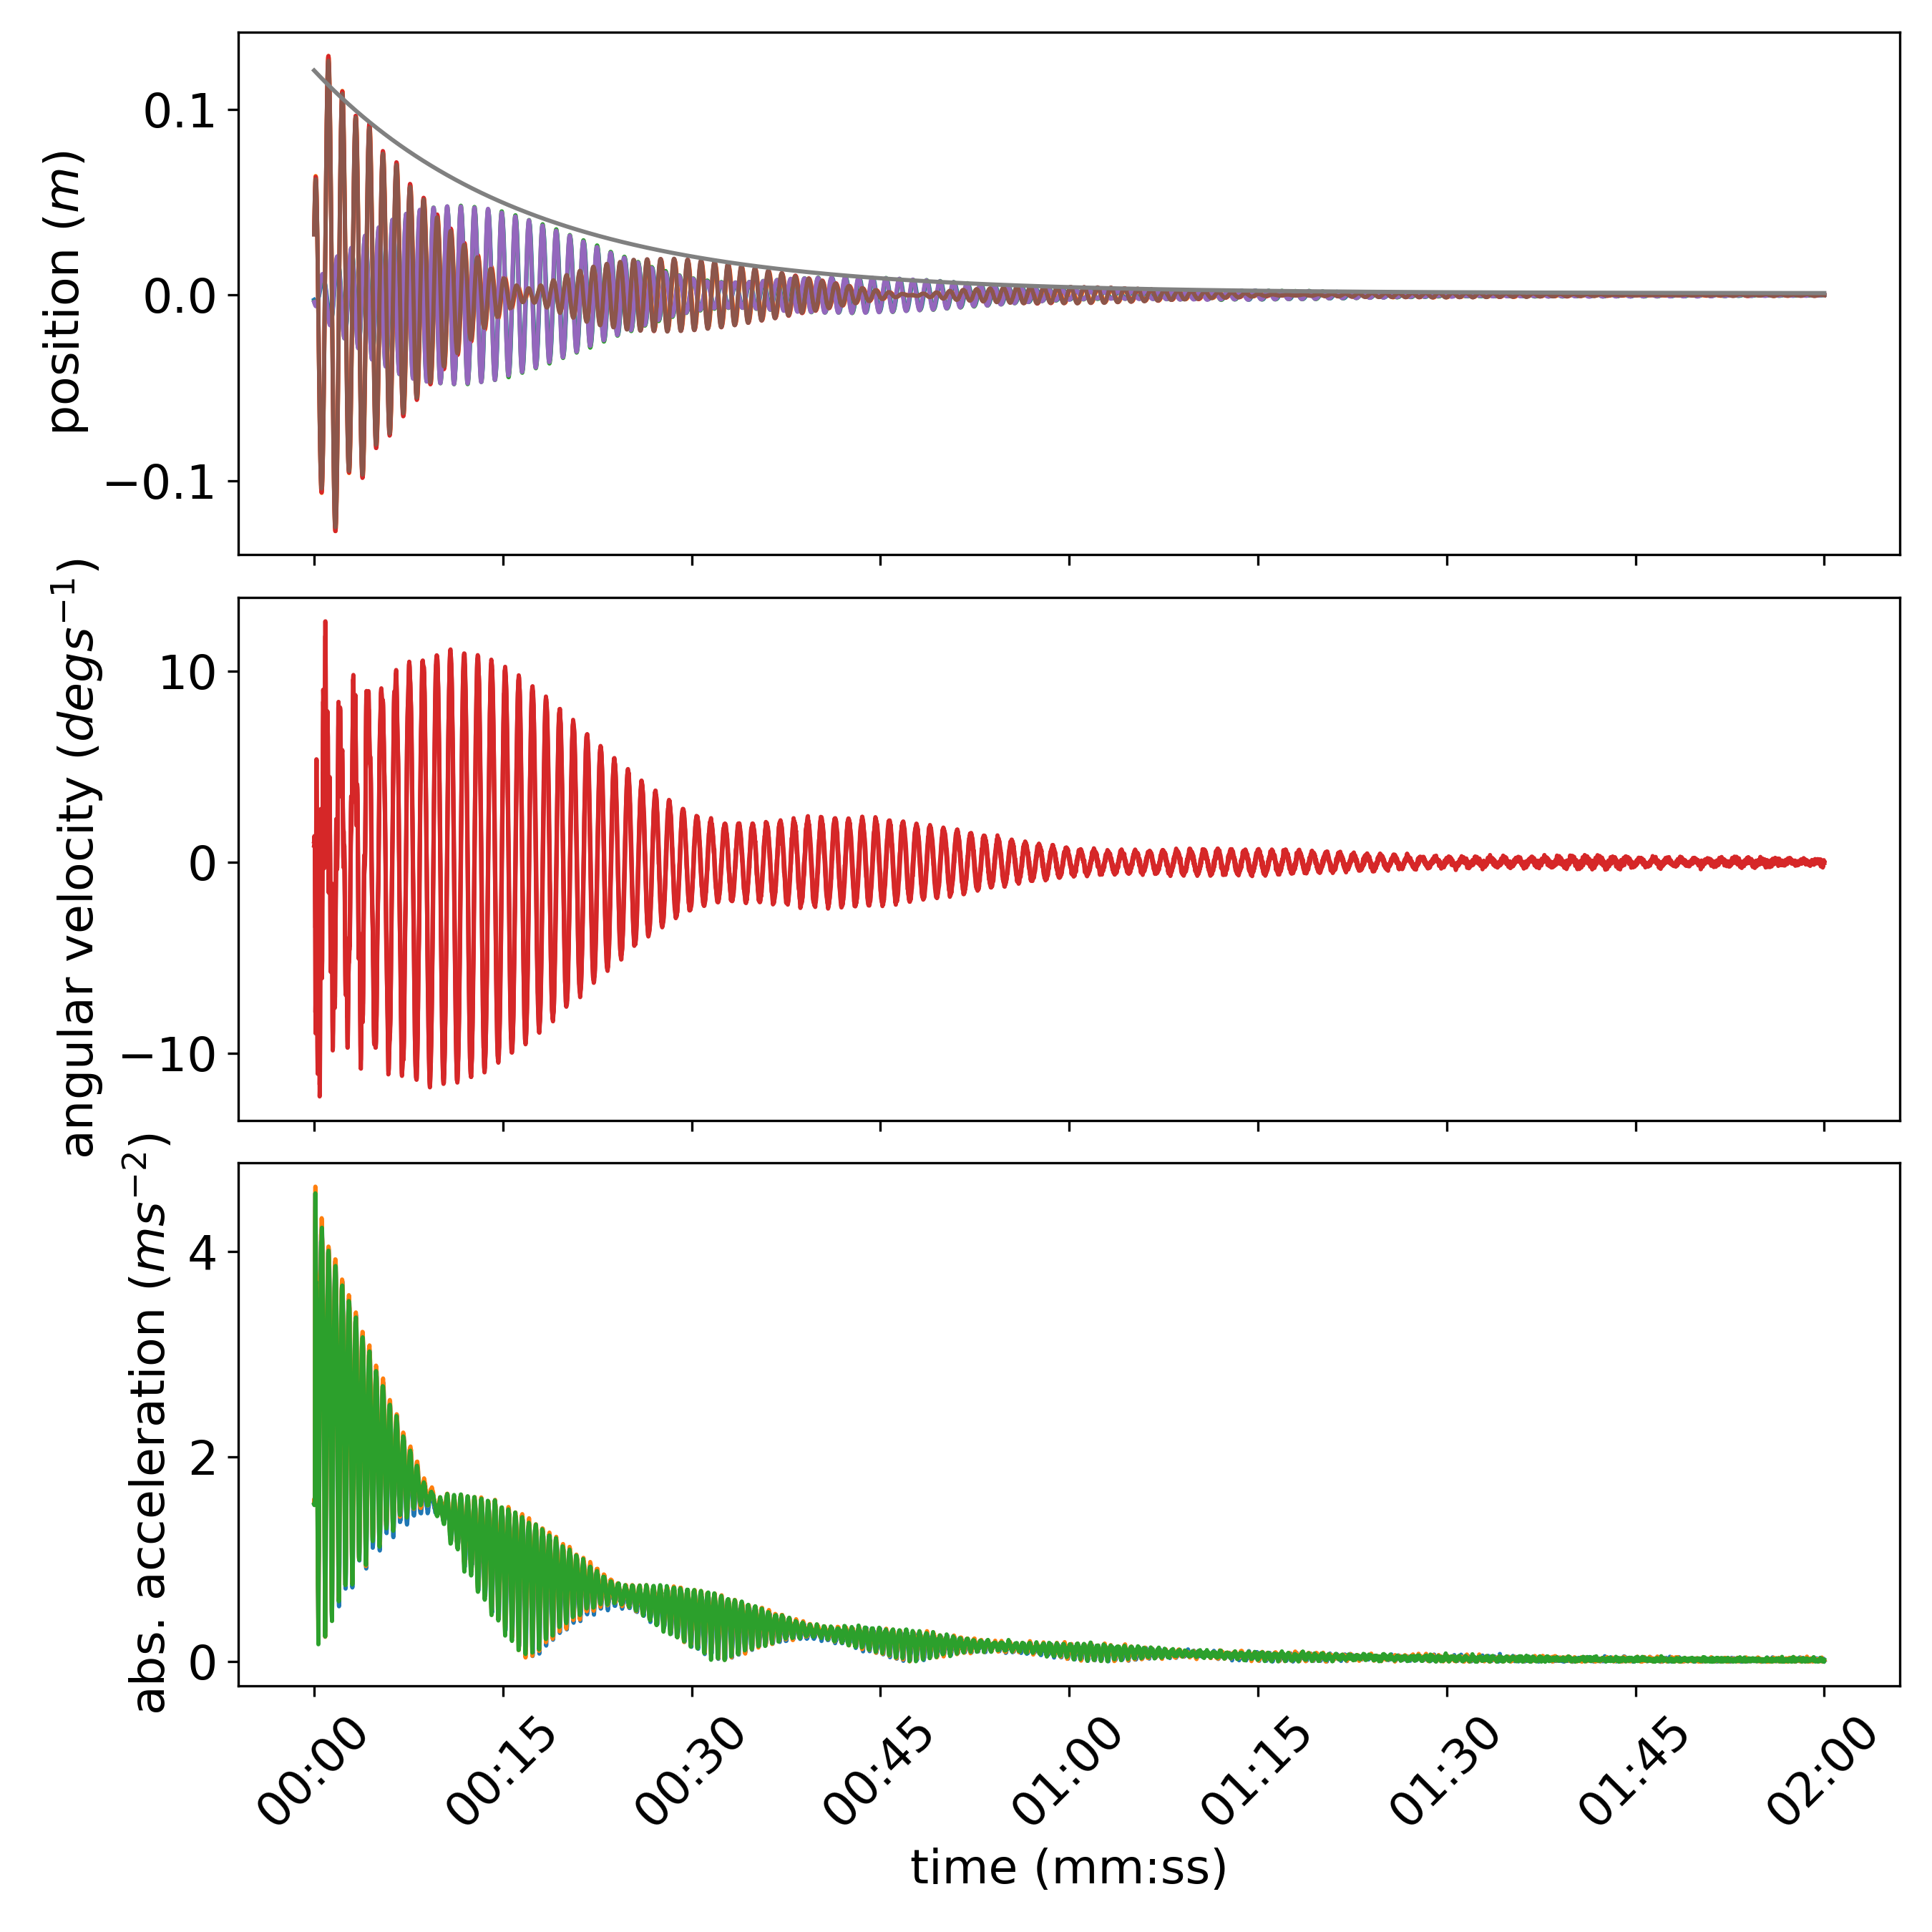
\includegraphics[width=\textwidth]{../results/experiment/high_mass_acceleration.png}
        \caption{}
        % \caption{Scatter diagram for mean deflection $d_{10}$ and significant wave height $H_{S10}$. The linear fit is shown as a blue line.}
        \label{fig:high-mass:acc}
    \end{subfigure}
    \begin{subfigure}[b]{0.45\textwidth}
        \centering
        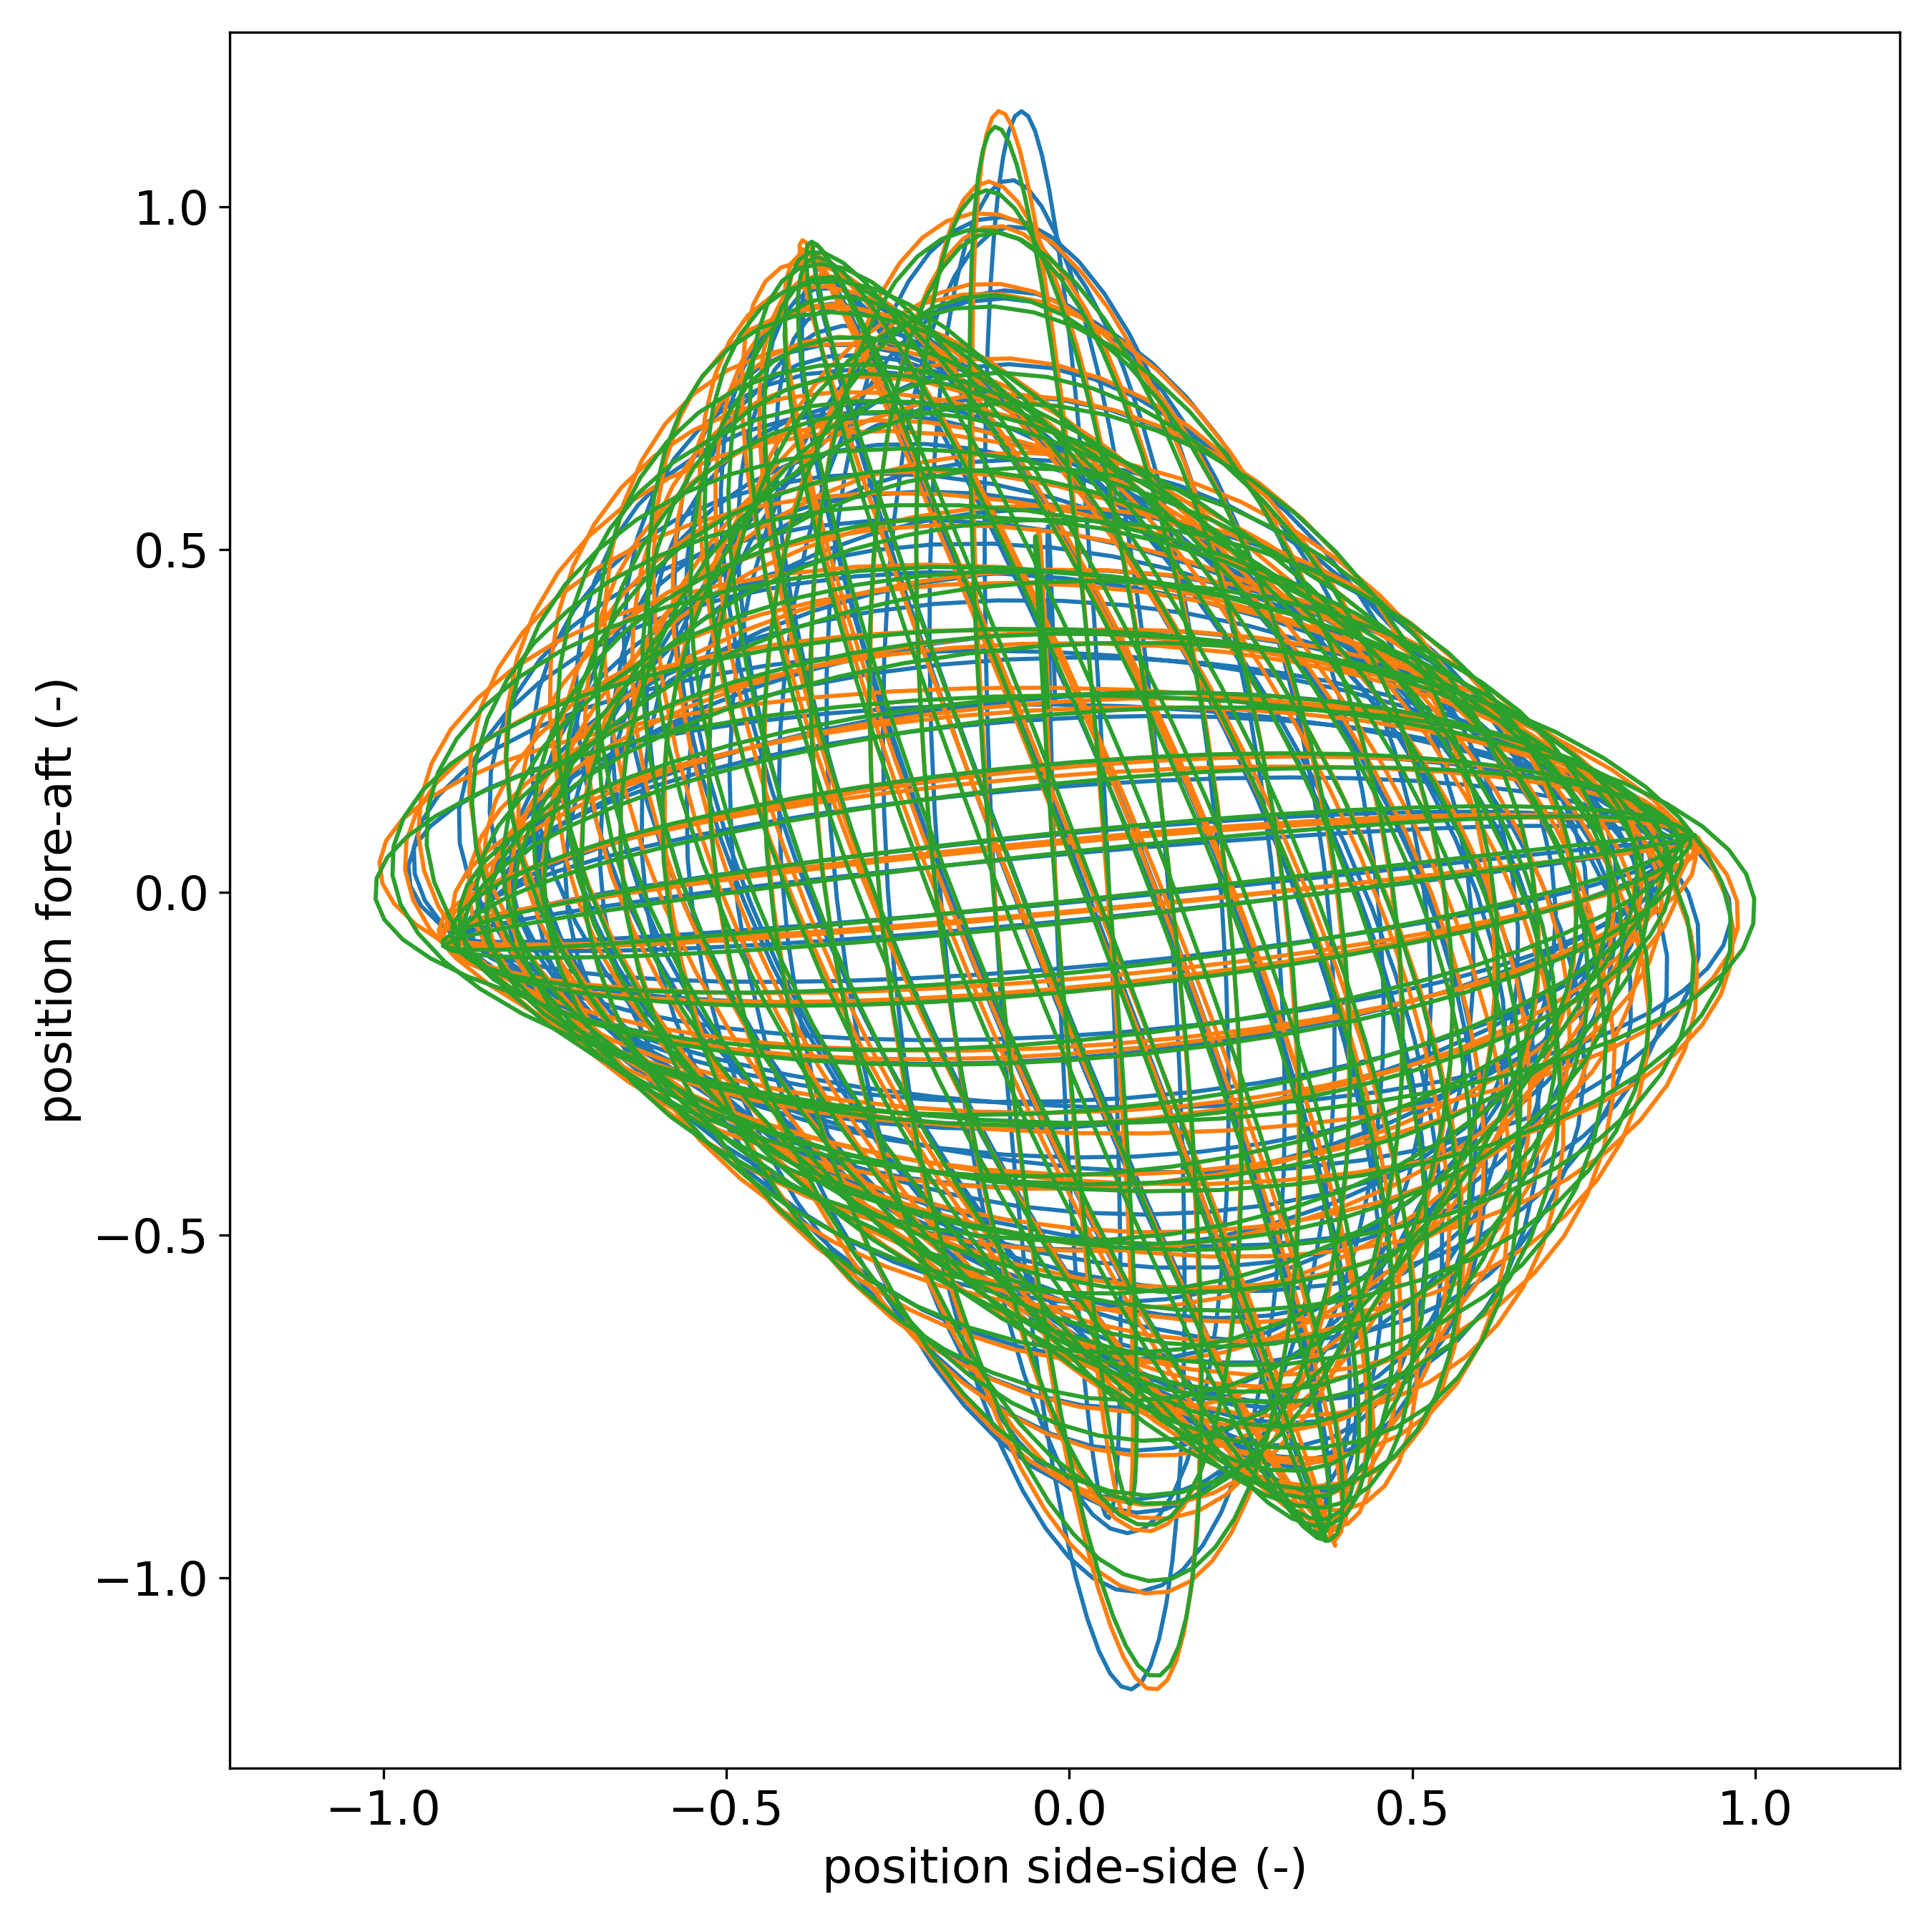
\includegraphics[width=\textwidth]{../results/experiment/high_mass_orbit.png}
        \caption{}
        % \caption{Scatter diagram for mean deflection $d_{10}$ and significant wave height $H_{S10}$. The linear fit is shown as a blue line.}
        \label{fig:high-mass:orbit}
    \end{subfigure}
    
    
    \caption{Accelerations, angular velocity and absolute acceleration (left) and Lissajous figures (orbits) for the high mass scenario.}
    \label{fig:high-mass}
\end{figure*}

It becomes apparent, that the area enclosing all observed orbits is a function of the eccentric mass. In the case of the medium mass scenario, the area is almost quadratic, whereas for the low and high mass scenarios the area is more distorted. For each mass scenario, three runs of the experiment are shown, and the observed orbits are in close resemblance between consecutive runs. With increasing mass, decay is slower. In all three mass scenarios, torsion of the eccentric mass around the rod's main axis can be observed. In the case of the low mass scenario, the maximum torsion rate occurs right at the beginning of the signal and seems to monotonically decrease. For the medium and high mass scenario, a distinct increase in torsion rate can be observed. This increase is accompanied by an increase in vibration perpendicular to the initial displacement direction.

\clearpage

\autoref{fig:spectrum} Shows the fast Fourier transform for the two transversal acceleration directions and the angular velocity. Three distinct peaks can be observed, each corresponding to one mass scenario; the lowest frequency corresponds to the highest mass scenario. 

\begin{figure}[ht]
    \centering
    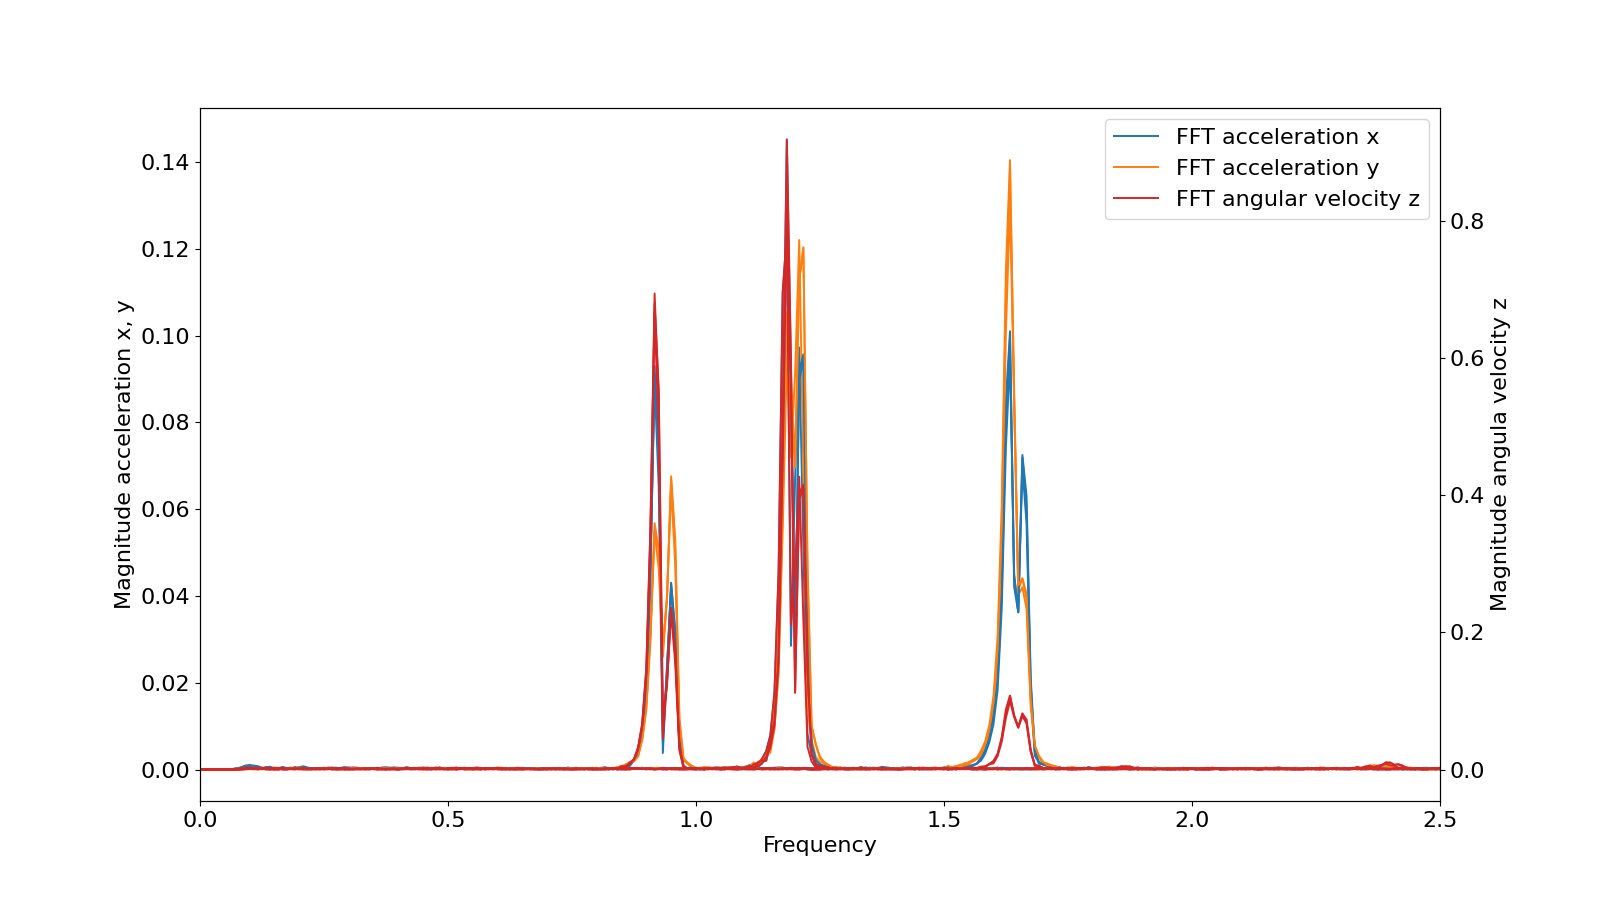
\includegraphics[width=0.5\linewidth]{../results/experiment/spectrum.png}
    \caption{Fast-Fourier transform of the two transversal accelerations and the angular velocity around the rod's main axis. The three distinct peaks each represent one mass scenario, with the left-most peak corresponding to the highest eccentric mass.}
    \label{fig:spectrum}
\end{figure}

\clearpage

\section{Finite-Element Simulations of a Cantilevered Beam}
\label{sec:simulations}

\subsection{Simulation Setup}

A numerical model based on the simplified system shown in Figure \autoref{fig:loading} was created using MATLAB, presented in Figure \autoref{fig:fea:model}. The cantilevered beam was modelled as a hollow cylinder made of  homogeneous linear elastic material and with a constant cross-section along its length, supported by linear uncoupled springs. The nacelle was modelled as a concentrated mass with inertia and a point mass with eccentricity in both the horizontal and the vertical plane.

\begin{figure}[ht]
    \centering
    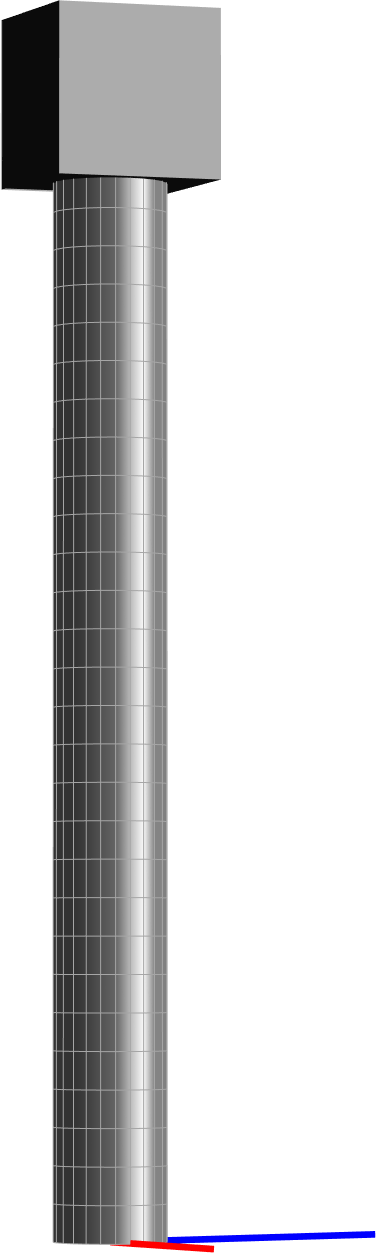
\includegraphics[width=0.5\linewidth]{figures/FEModel.png}
    \caption{FE model}
    \label{fig:fea:model}
\end{figure}

The equations of motion of the undamped system, in the following form,

\begin{equation}
    \mathbf{\bar{M}}\ddot{\mathbf{u}}+\mathbf{\bar{K}}\mathbf{u} = \mathbf{\bar{f}}
    \label{eq:fea:system}
\end{equation}

were obtained by superposition of the equations of motions of the concentrated and eccentric point mass ($ \mathbf{\bar{M}} = \mathbf{M}_{m_c} + \mathbf{M}_{m_e}$) at the free end of the cantilevered beam, the equations for the support springs and the equations for the cantilevered beam itself. The cantilevered beam was modelled based on linear one-dimensional finite element equations with six degrees of freedom in the global coordinate system. Euler Bernoulli beam theory was used to deal with bending. Using a rotation matrix based on Tait–Bryan angles, the equations of motions for the concentrated, eccentric top mass were derived by applying the Euler Lagrange equation. Using Taylor series for linearization, the  mass matrix (\autoref{eq:fea:Mtop}), stiffness matrix (\autoref{eq:fea:K_m_ecc}) and gravitational force ( \autoref{eq:fea:Fstat}) were found for the six global degrees of freedom. The stiffness matrix of the support springs is presented in \autoref{eq:fea:K_fnd}. 

\begin{small}
    \begin{equation}
        \mathbf{M}_{m_c} + \mathbf{M}_{m_e}  = 
        \begin{bmatrix}
         m_{e}+m_{c}   & 0             & 0             & 0                                             & m_{e}\,z_{e}                                  & -m_{e}\,y_{e}        \\ 
         0             & m_{e}+m_{c}   & 0             & -m_{e}\,z_{e}                                 & 0                                             & m_{e}\,x_{e}         \\ 
         0             & 0              & m_{e}+m_{c}   & m_{e}\,y_{e}                                  & -m_{e}\,x_{e}                                 & 0                    \\ 
         0             & -m_{e}\,z_{e} & m_{e}\,y_{e}  & I_{c}+\left({z_{e}}^2+{y_{e}}^2\right)\,m_{e} & -m_{e}\,x_{e}\,y_{e}                          & -m_{e}\,x_{e}\,z_{e} \\ 
         m_{e}\,z_{e}  & 0             & -m_{e}\,x_{e} & -m_{e}\,x_{e}\,y_{e}                          & I_{c}+\left({z_{e}}^2+{x_{e}}^2\right)\,m_{e} & -m_{e}\,y_{e}\,z_{e} \\
         -m_{e}\,y_{e} & m_{e}\,x_{e}  & 0             & -m_{e}\,x_{e}\,z_{e}                          & -m_{e}\,y_{e}\,z_{e}                          & I_{c}+\left({y_{e}}^2+{x_{e}}^2\right)\,m_{e} 
        \end{bmatrix}
        \label{eq:fea:Mtop}
    \end{equation}
\end{small}

The mass of the cantilevered beam is $m_c$ and the eccentric mass is referred to by $m_e$. 

\begin{small}
    \begin{equation}
        \mathbf{K}_{m_e} =
        \begin{bmatrix}
       0 & 0 & 0 &         0        &        0         & 0 \\ 
       0 & 0 & 0 &         0        &        0         & 0 \\ 
       0 & 0 & 0 &         0        &        0         & 0 \\ 
       0 & 0 & 0 & -g\,m_{e}\,z_{e} &        0         & 0 \\ 
       0 & 0 & 0 &         0        & -g\,m_{e}\,z_{e} & 0 \\ 
       0 & 0 & 0 &         0        &        0         & 0
        \end{bmatrix}
        \label{eq:fea:K_m_ecc}
    \end{equation}
\end{small}

\begin{small}
    \begin{equation}
        \mathbf{f}_{m_c} + \mathbf{f}_{m_e} = 
        \begin{bmatrix}
         0\\ 0\\ -g(\,m_{e}+m_{c})\\ -g\,m_{e}\,y_{e}\\ g\,m_{e}\,x_{e} \\ 0
        \end{bmatrix}
        \label{eq:fea:Fstat}
    \end{equation}
\end{small}

\begin{small}
    \begin{equation}
        \mathbf{K}_{fnd} =
        \begin{bmatrix}
         k_{x} &     0 & 0     & 0         & 0           & 0         \\ 
         0     & k_{y} & 0     & 0         & 0           & 0         \\
         0     & 0     & k_{z} & 0         & 0           & 0         \\
         0     & 0     & 0     & k_{\phi } & 0           & 0         \\
         0     & 0     & 0     & 0         & k_{\theta } & 0         \\ 
         0     & 0     & 0     & 0         & 0           & k_{\psi } 
        \end{bmatrix}
        \label{eq:fea:K_fnd}
    \end{equation}
\end{small}

As loads, gravitational force and an initial deformation due to a horizontal force applied at the centre of the top of the cantilevered beam were considered. Multiple combinations of amplitude and direction of the initial deformation were simulated, as well as load cases with and without gravitational force. In addition, the top mass and its vertical and horizontal eccentricity were varied. To account for limitations due to linearization of the numerical model, small initial deformations were applied.

\subsection{Simulation Results}

The response to gravitational force and an initial deformation due to a horizontal force applied at the top of the  cantilevered beam with an angle of 45\textdegree regarding the eccentricity of the point mass is presented in Figure \autoref{fig:fea:lissa_simu_results}. The pattern found in the simulations (\autoref{fig:fea:lissa_orbits}) appear to be quite similar to the pattern found in the experiments, as presented in Figure \autoref{fig:high-mass:orbit}.

To compare the effect of gravitational force and vertical eccentricity of the point mass, the response  for a load cases with- and without gravitational force and vertical eccentricity are presented in Figure \autoref{fig:fea:simres_gravitational_force_comparison}. These responses result from simulations with a short time span and would have shown a similar pattern to the response presented in Figure\autoref{fig:fea:lissa_simu_results}, (\autoref{fig:fea:lissa_orbits}), if the simulation time span was extended. 

\begin{figure*}
\centering
    \begin{subfigure}[b]{0.45\textwidth}
        \centering
        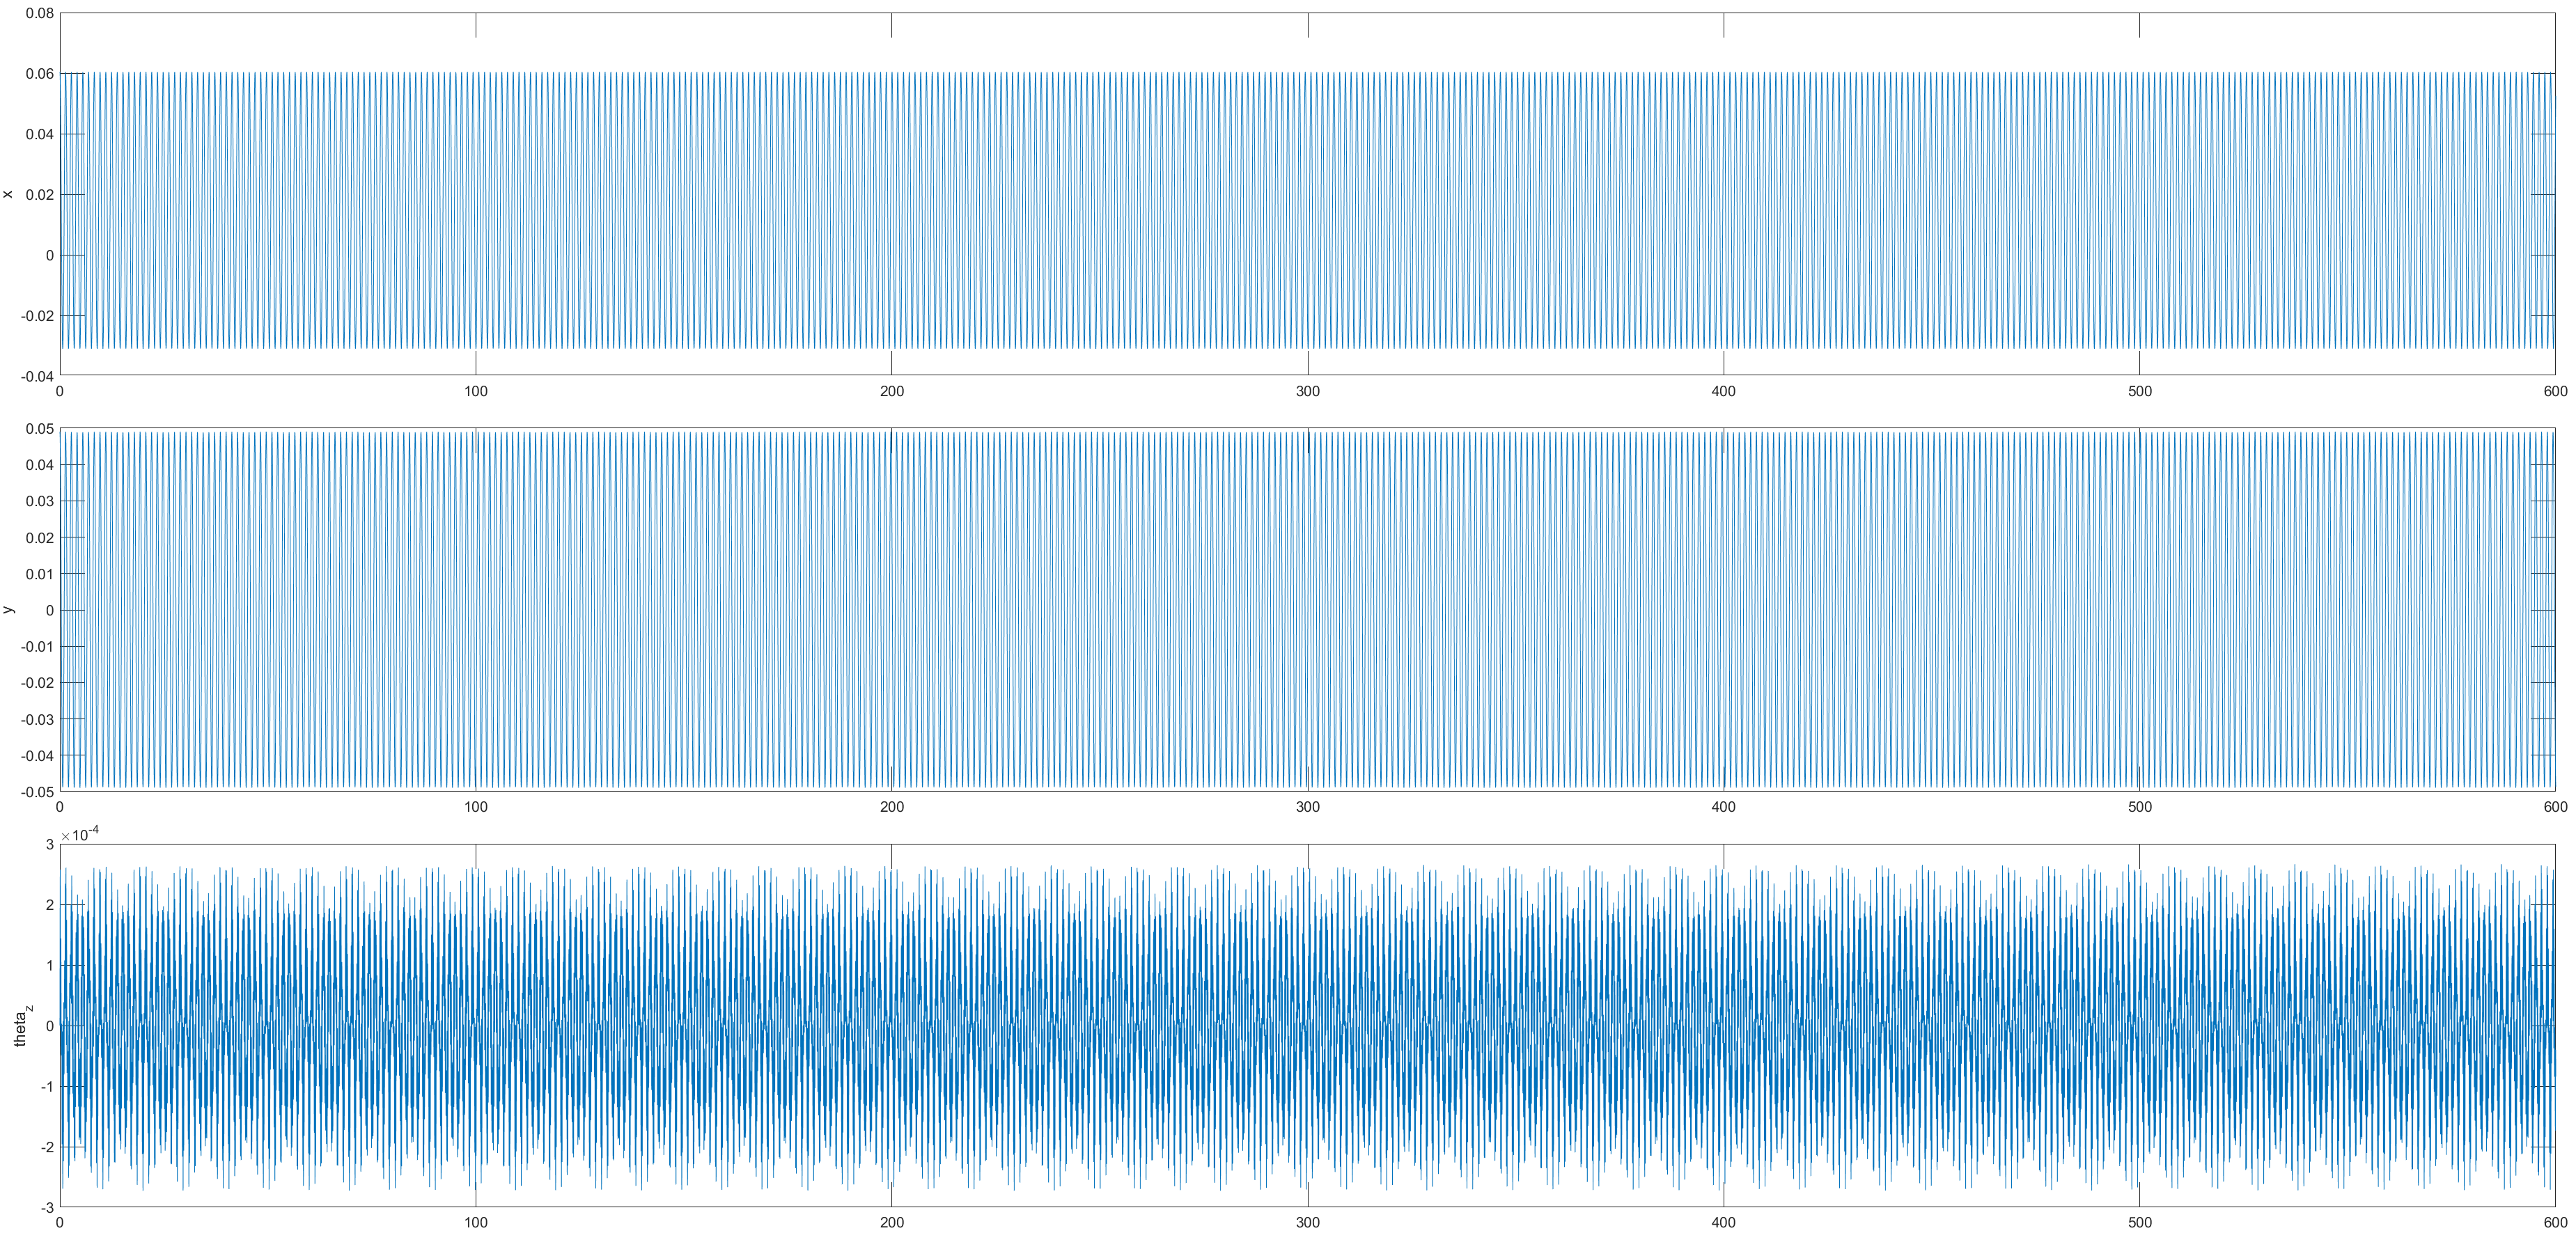
\includegraphics[width=\textwidth]{figures/FEA_simu_Lissa_Displacement.png}
        % \caption{}
        % \caption{Scatter diagram for mean deflection $d_{10}$ and significant wave height $H_{S10}$. The linear fit is shown as a blue line.}
        \caption{\small{Horizontal displacement and rotation about vertical axis}}
        \label{fig:fea:lissa_displ}
    \end{subfigure}
    \begin{subfigure}[b]{0.45\textwidth}
        \centering
        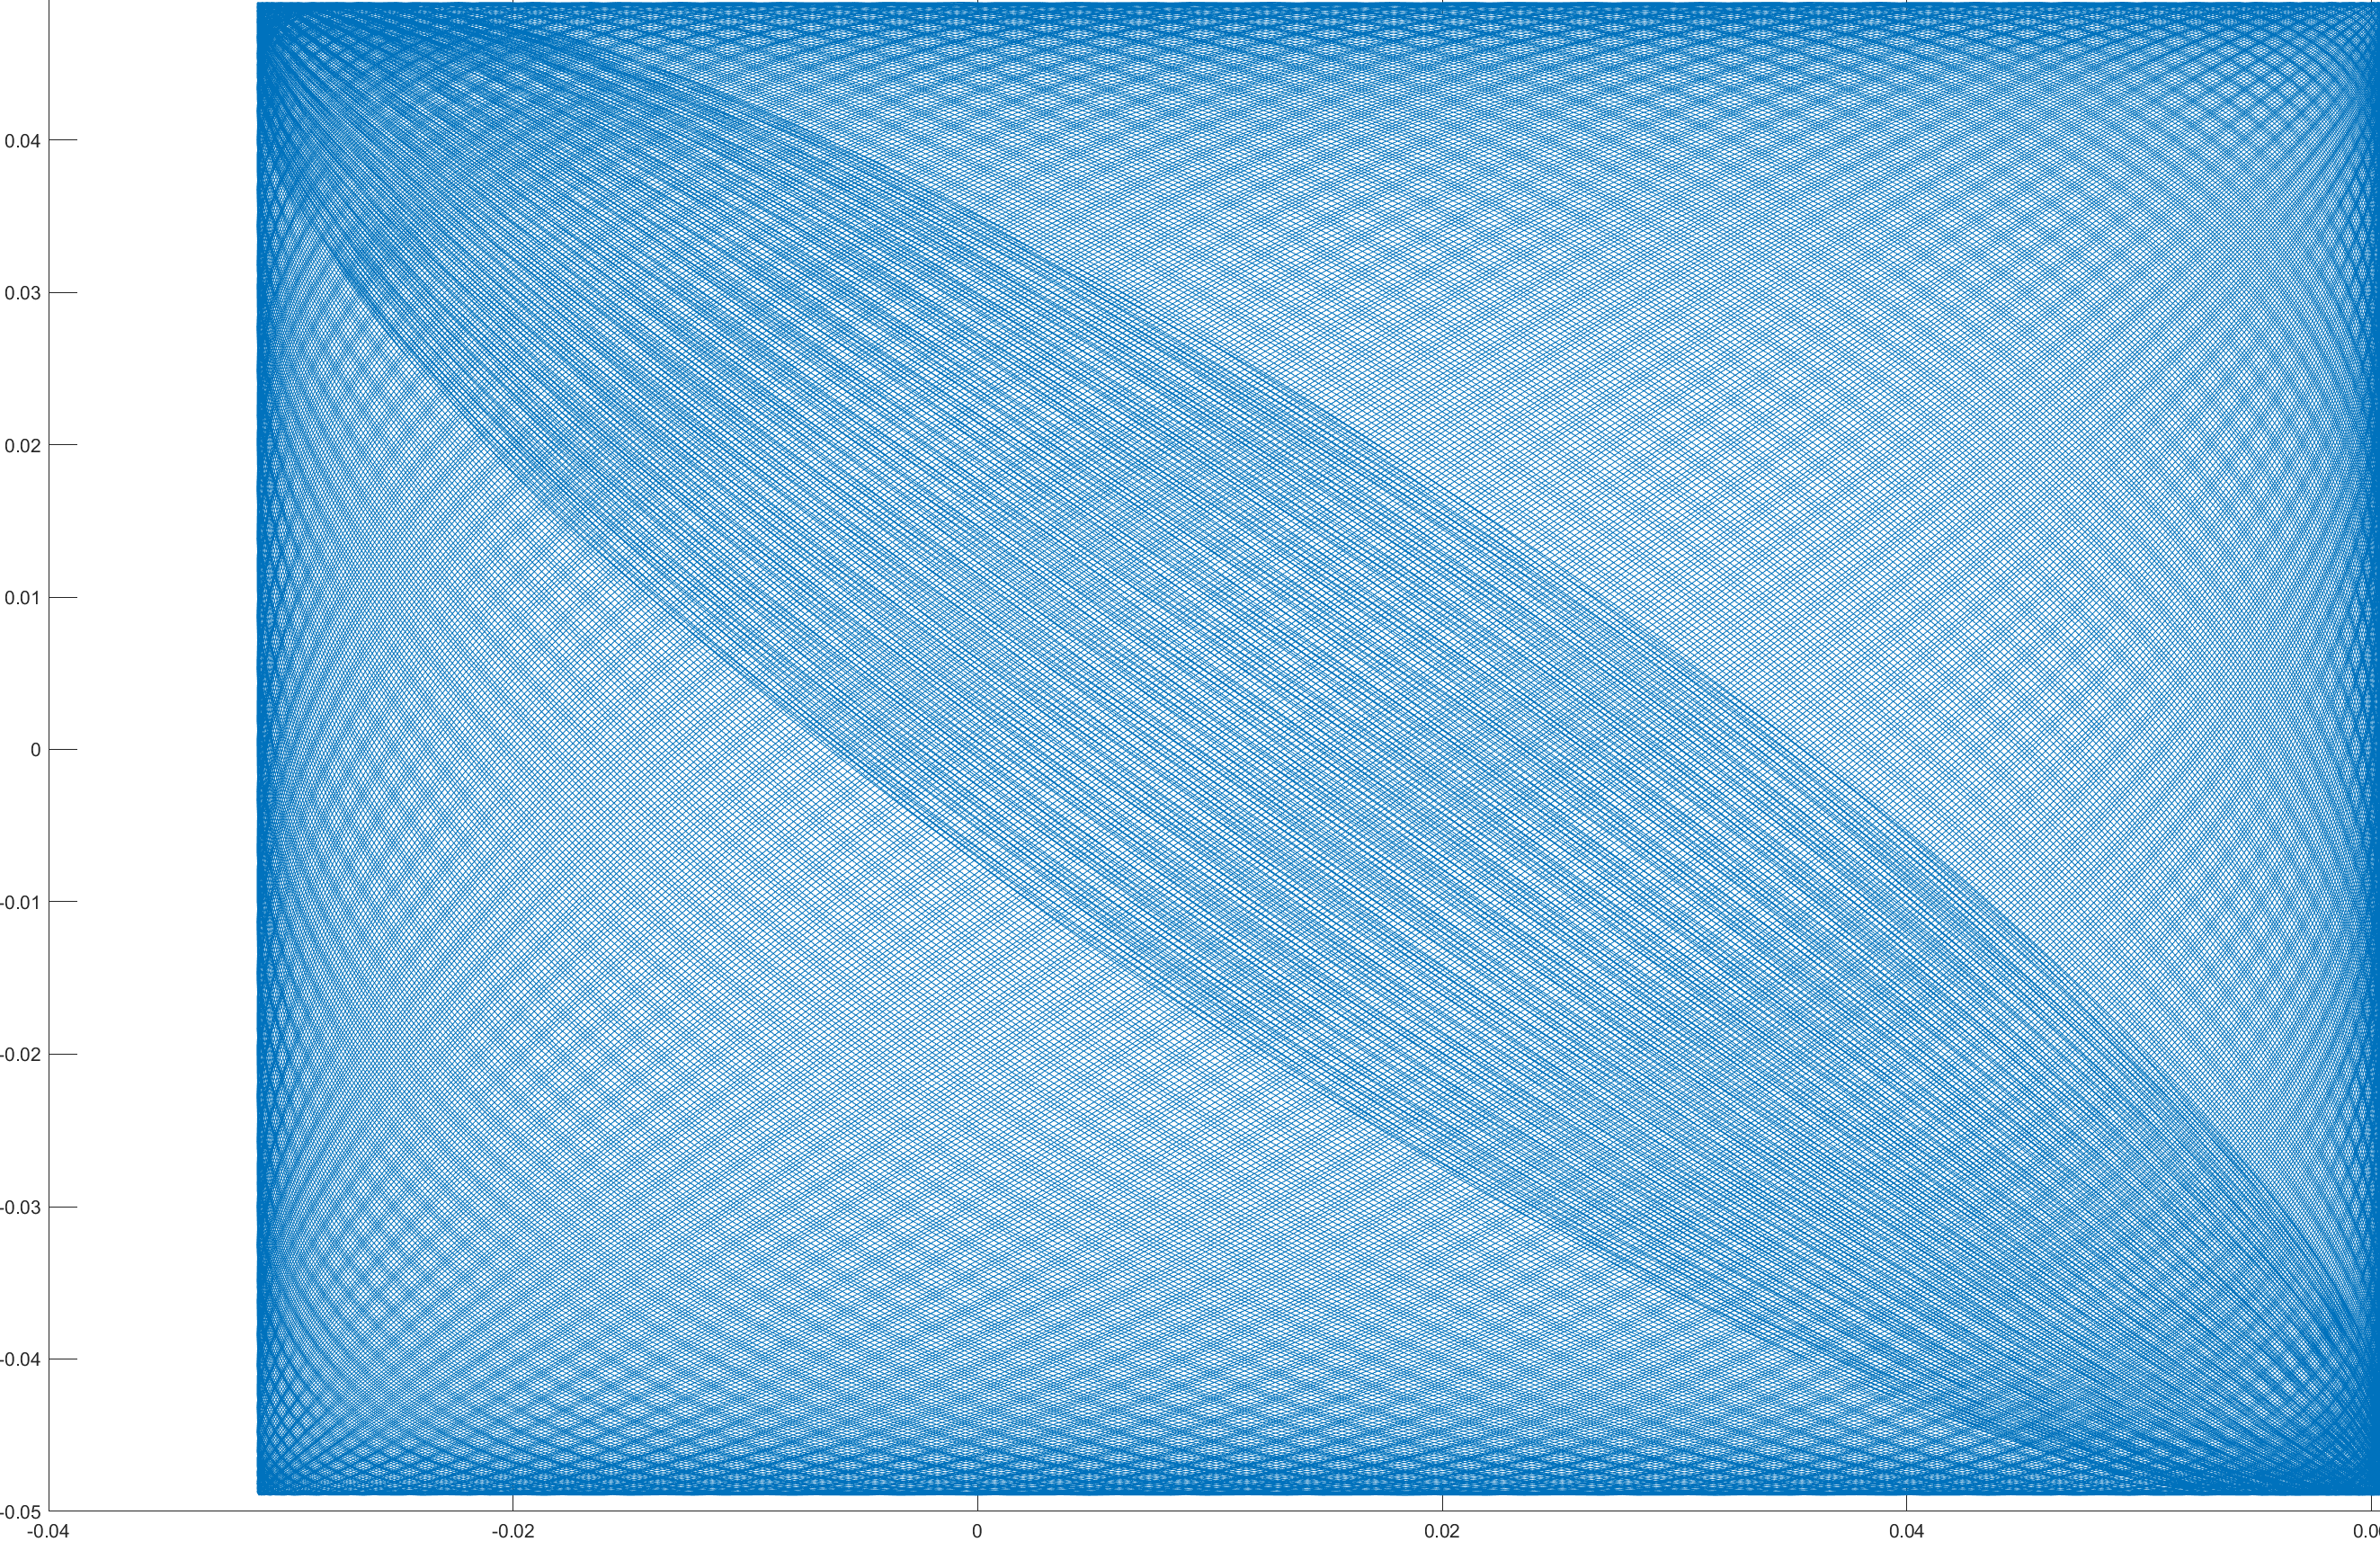
\includegraphics[width=\textwidth]{figures/FEA_simu_Lissa_Orbits.png}
        \caption{\small{Formation of obits in the horizontal plane}}
        % \caption{Scatter diagram for mean deflection $d_{10}$ and significant wave height $H_{S10}$. The linear fit is shown as a blue line.}
        \label{fig:fea:lissa_orbits}
    \end{subfigure}
\caption{FE simulation results: Lissajous curve}
    \label{fig:fea:lissa_simu_results}
\end{figure*}


\begin{figure*}
\centering
    \begin{subfigure}[b]{0.45\textwidth}
        \centering
        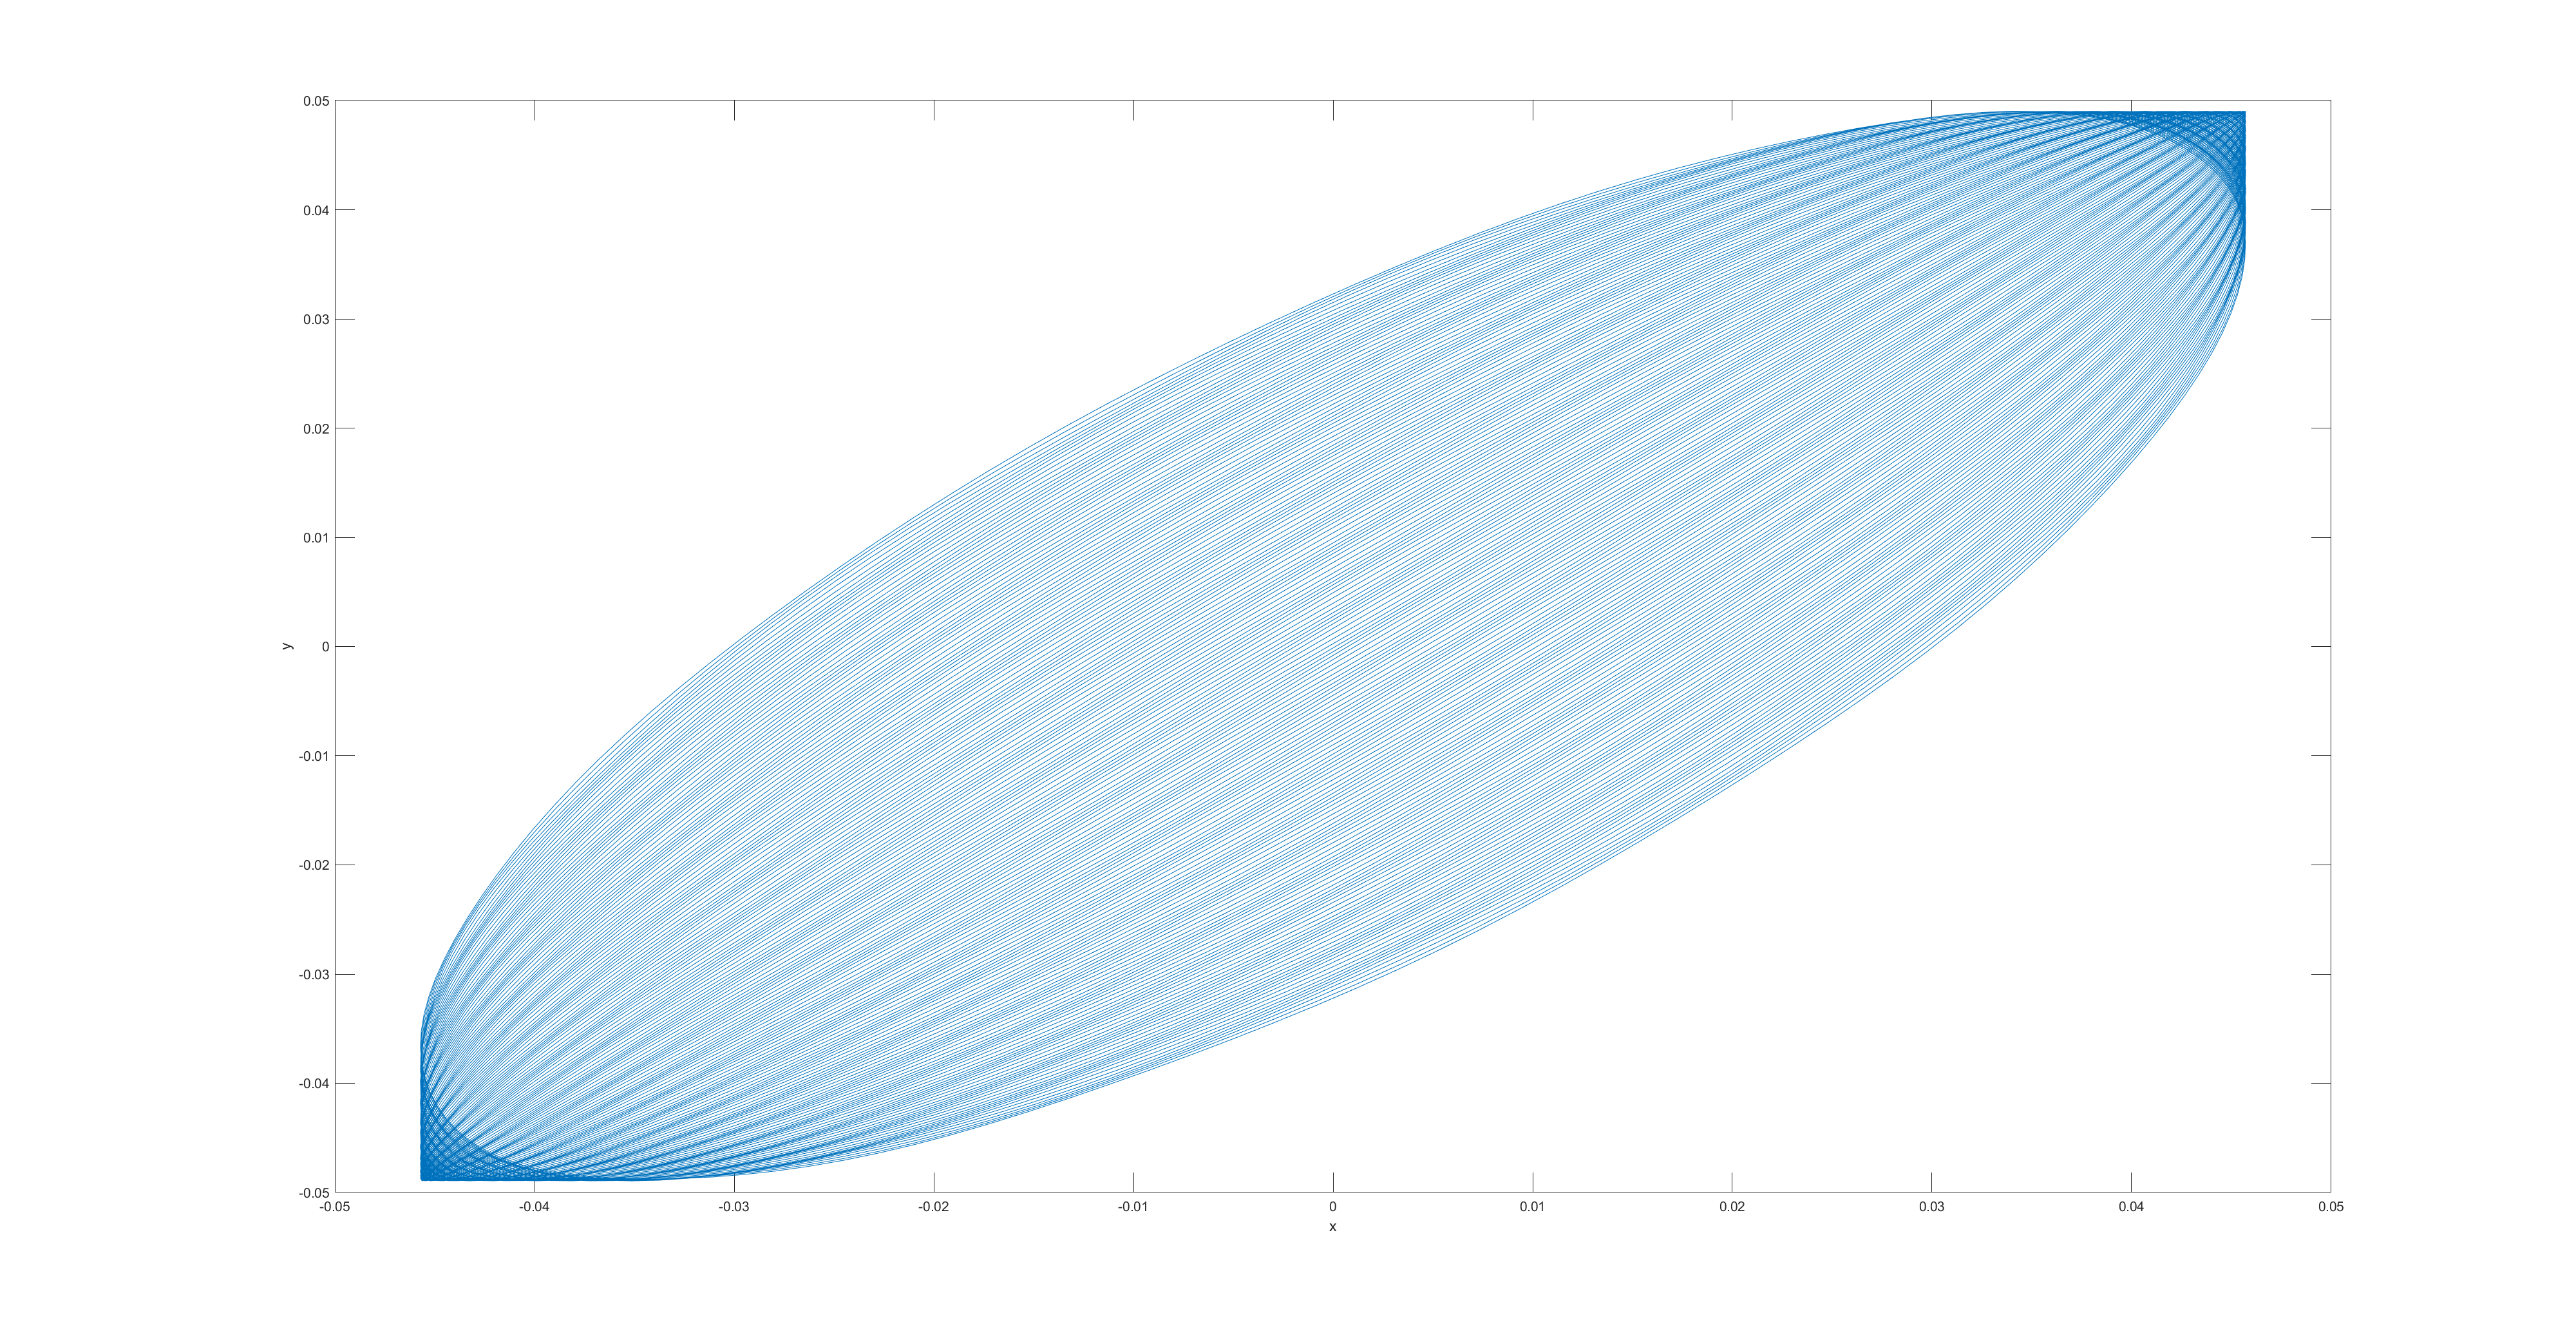
\includegraphics[width=\textwidth]{figures/FEA_simu_Orbits_No_grav.png}
        % \caption{}
        % \caption{Scatter diagram for mean deflection $d_{10}$ and significant wave height $H_{S10}$. The linear fit is shown as a blue line.}
        \caption{\small{Without gravitational force}}
        \label{fig:fea:simres_nograp}
    \end{subfigure}
    \begin{subfigure}[b]{0.45\textwidth}
        \centering
        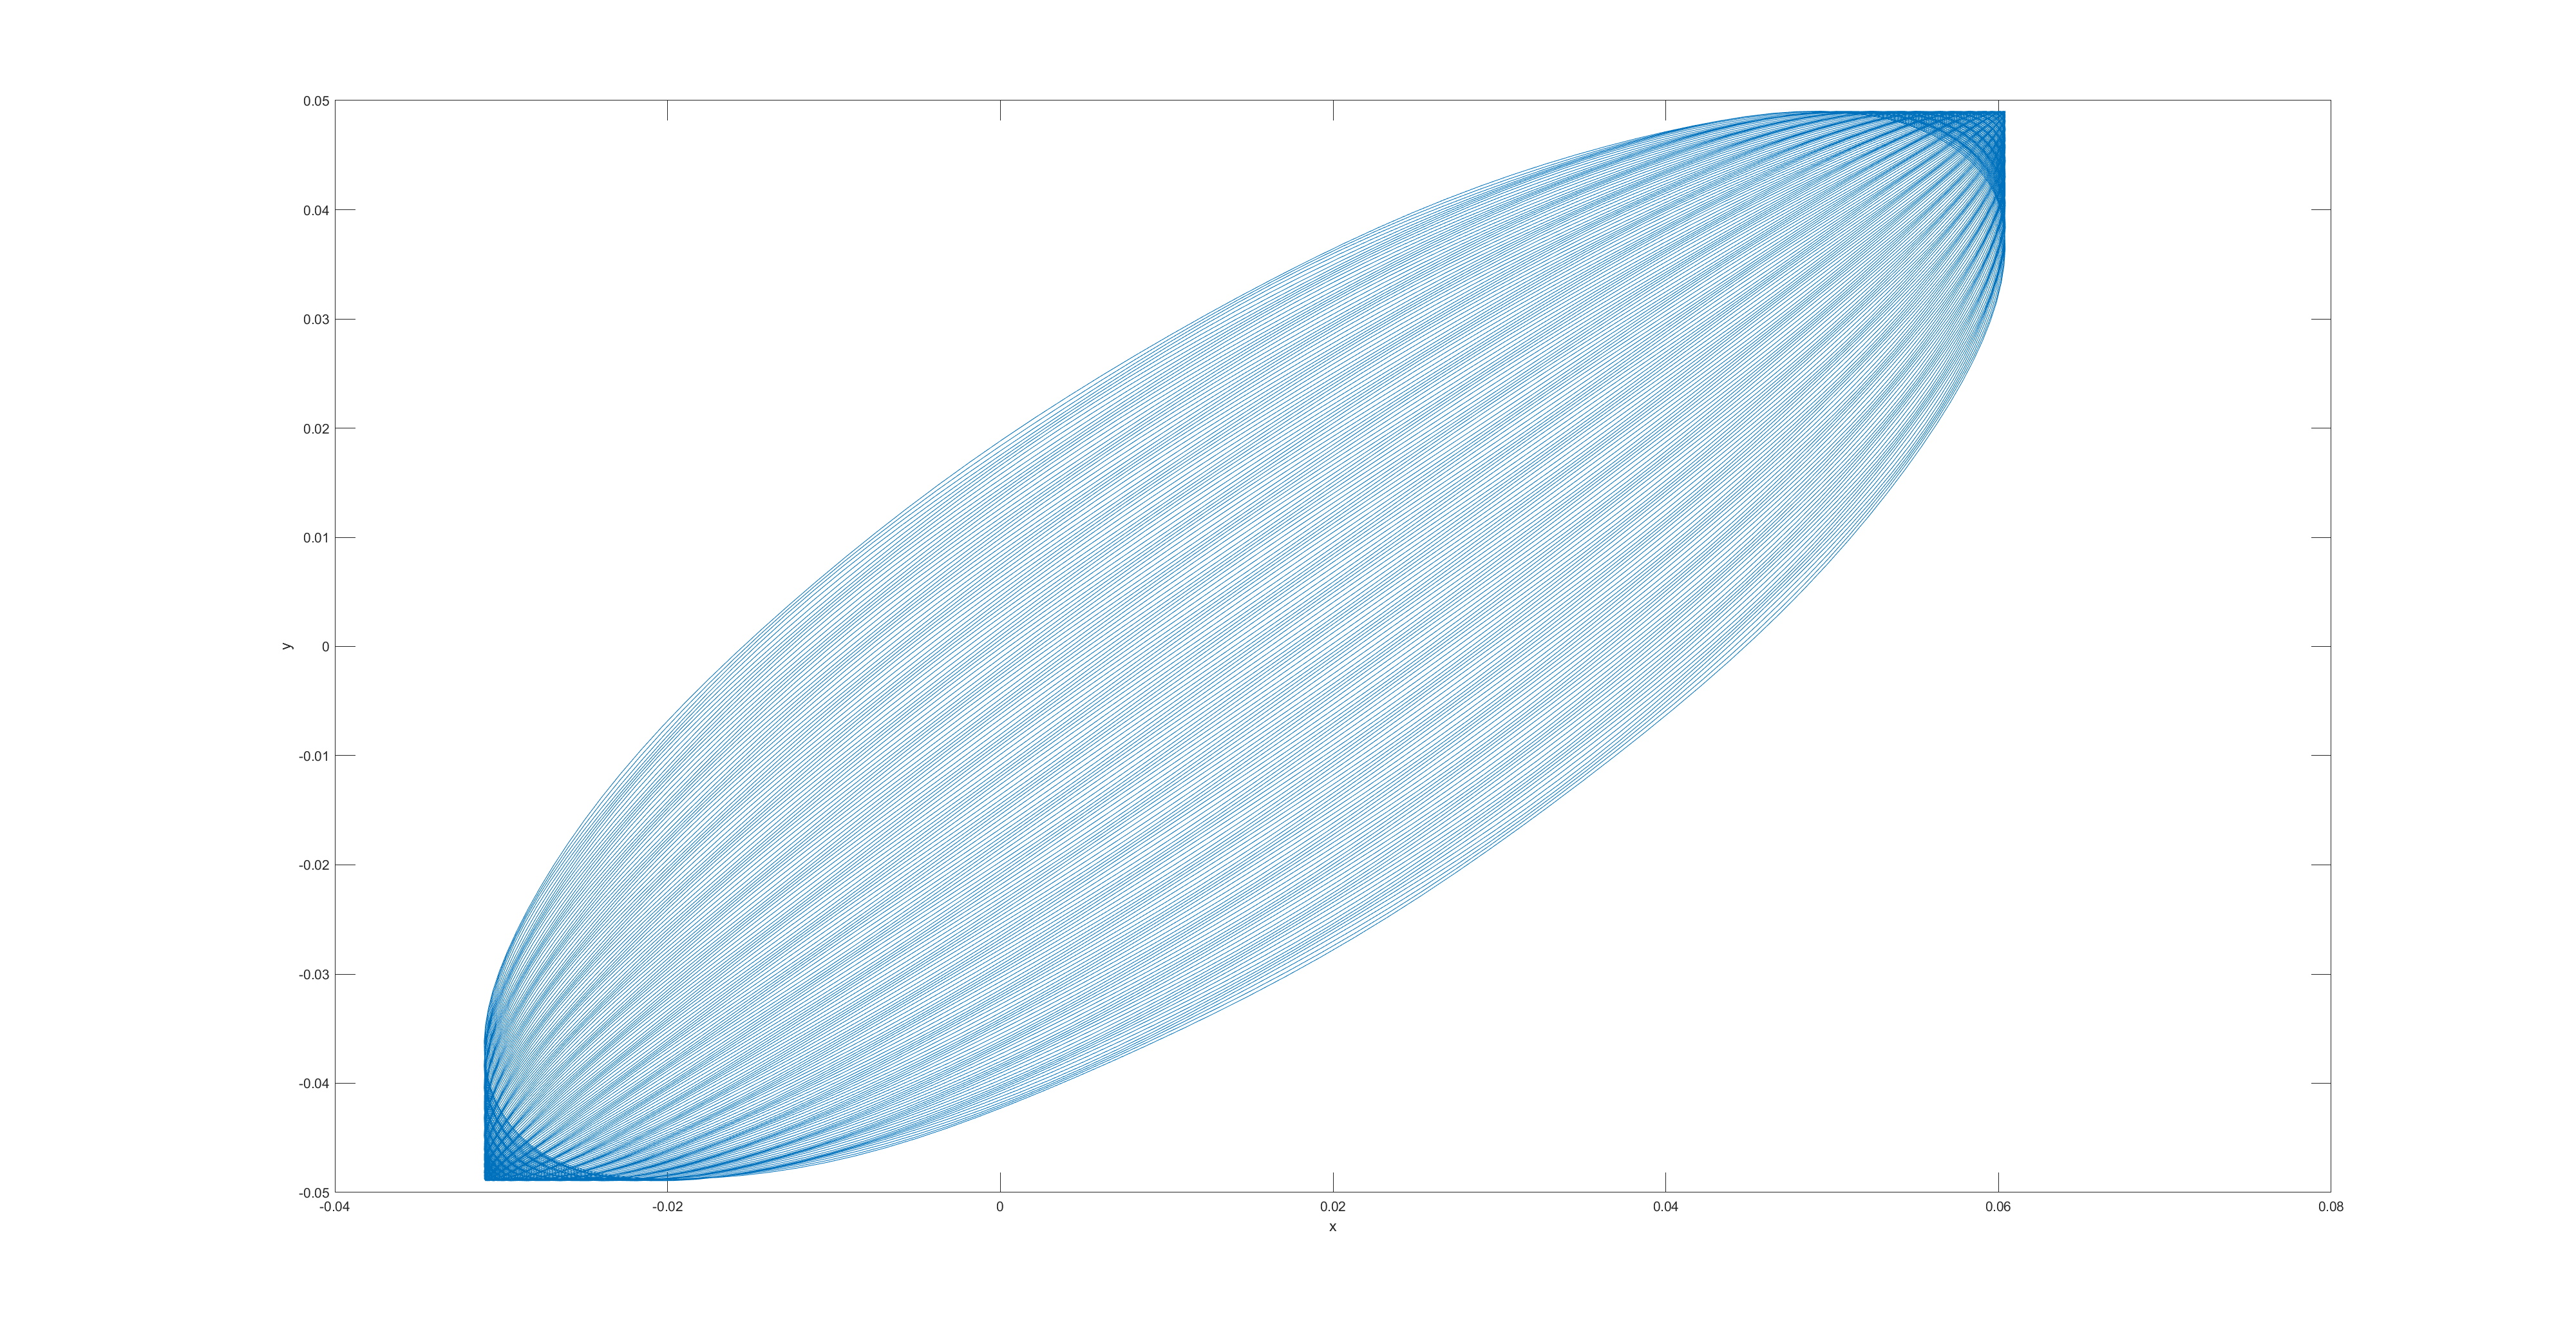
\includegraphics[width=\textwidth]{figures/FEA_simu_Orbits_With_grav.png}
        \caption{\small{With gravitational force}}
        % \caption{Scatter diagram for mean deflection $d_{10}$ and significant wave height $H_{S10}$. The linear fit is shown as a blue line.}
        \label{fig:fea:simres_withgrav}
    \end{subfigure}
\caption{FE simulation results: with and without gravitational force}
    \label{fig:fea:simres_gravitational_force_comparison}
\end{figure*}

\clearpage

\section{A vibration model with three degrees of freedom}
\label{sec:3dof}

A common approach to study vibrations is to reduce the real system into a simplified model that consists of discrete components. In this approach, one aims to describe the real system as simple as possible to generate the main dynamics of the real system. Many vibration phenomena can be sufficiently described with systems with only one or two degrees of freedom. Here, we present a model with three degrees of freedom that seems to capture the main dynamics of the real system.
\par 
We model the real system in two dimensions (\autoref{fig:3dof-system}). The tower's bending is modelled as a linear spring, which is connected to a fixed point, which represents the tower's foundation, and to a first body, which represents the tower's top section. The tower's torsion is modelled with a torsional spring that connects a second body with a fixed angle in the inertial reference frame. This second body is pinned to the first body such that it translates with the first body, but rotates freely. Consequently, the system's three degrees of freedom are: the first body's position in $x$ and $y$ direction and the second body's orientation.
\par 
By applying the physical laws of conservation of linear and angular momentum, we derived the equations of motions for the system (a derivation is available as supplemental material). The system's equations of motion read:
\begin{equation}
    (m_1 + m_2) \ddot{x} - \cos(\theta) m_2 d \ddot{\theta} + \sin(\theta) m_2 d \dot{\theta}^2 + k_1 x = 0,\label{eq:eom-x}
\end{equation}
\begin{equation}
    (m_1 + m_2) \ddot{y} - \sin(\theta) m_2 d \ddot{\theta} - \cos(\theta) m_2 d \dot{\theta}^2 + k_1 y = 0,\label{eq:eom-y}
\end{equation}
\begin{equation}
    (I_{zz} + m_2 d^2)\ddot{\theta} - \cos(\theta) m_2 d \ddot{x} - \sin(\theta)m_2 d \ddot{y} + k_2 \theta = 0.\label{eq:eom-theta}
\end{equation}

The equations can be arranged to have only acceleration on the left hand side:
\begin{equation}
    \ddot{x} = \frac{1}{m_1 + m_2} \left( \cos(\theta) m_2 d \ddot{\theta} - \sin(\theta) m_2 d \dot{\theta}^2 - k_1 x \right),\label{eq:eom2-x}
\end{equation}
\begin{equation}
   \ddot{y} = \frac{1}{m_1 + m_2} \left(\sin(\theta) m_2 d \ddot{\theta} + \cos(\theta) m_2 d \dot{\theta}^2 - k_1 y \right),\label{eq:eom2-y}
\end{equation}
\begin{equation}
    \ddot{\theta} = \frac{1}{I_{zz} + m_2 d^2} \left(\cos(\theta) m_2 d \ddot{x} + \sin(\theta)m_2 d \ddot{y} - k_2 \theta \right) \label{eq:eom2-theta}
\end{equation}

Several terms couple translation ($x$ and $y$) with rotation ($\theta$): for example, the acceleration in the $x$ direction, $\ddot{x}$ is equal to terms that contain $\ddot{\theta}$ and $\dot{\theta}$ (\autoref{eq:eom2-x}). Such coupling terms are necssary to appear in the equation as otherwise only linear motion would be possible -- in other words, the mass would move back and forth on a straight line.
\par 
The translational acceleration is affected by the second mass' centrifugal and Euler forces. Centrifugal force acts in the $-\hat{r}$ direction and reads, 
\begin{equation}
    m_2 d \dot{\theta}^2,
\end{equation}
and Euler force acts in the $\hat{\theta}$ direction and reads
\begin{equation}
    m_2 d \ddot{\theta}.
\end{equation}
The equation for $\ddot{\theta}$ (\autoref{eq:eom2-theta}) was derived by applying conservation of angular momentum around the center of mass $G$. The force that acts at the location where the second body is pinned to the first body depend on the first body's acceleration in $x$ and $y$ direction such that there are also coupling terms with $\ddot{x}$ and $\ddot{y}$ in the equation for $\ddot{\theta}$  (\autoref{eq:eom2-theta}).
\par 
As expected, the equations also show that if $d=0$ the coupling terms disappear:
\begin{equation}
    (m_1 + m_2) \ddot{x} = - k_1 x,
\end{equation}
\begin{equation}
   (m_1 + m_2) \ddot{y} = - k_1 y,
\end{equation}
\begin{equation}
    I_{zz}\ddot{\theta} = - k_2 \theta.
\end{equation}

\begin{figure}
    \centering
    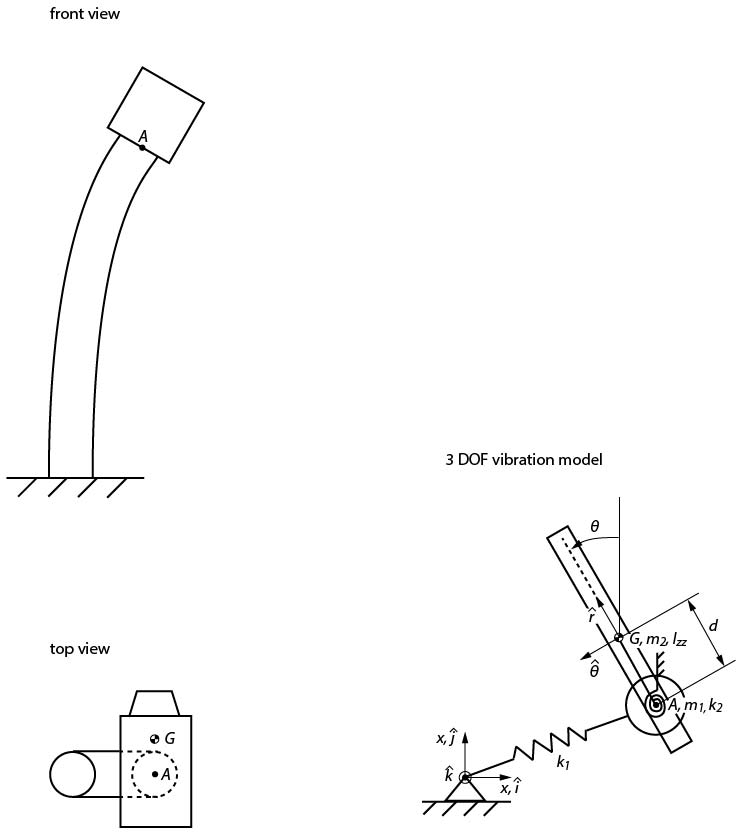
\includegraphics{figures/vibration_model.jpg}
    \caption{A vibration model with three degrees of freedom (DOF).}
    \label{fig:3dof-system}
\end{figure}

With parameter values similar as in the table top experiment, the vibration model leads to similar motions: Orbits with changing major axis direction appear (\autoref{fig:3dof-tabletop}). With parameters values similar to an offshore wind turbine in the hammerhead configuration (tower and nacelle installed, but not the blades yet), orbit direction changes do not occur. If the torsional stiffness is very high such that torsional motions are very low, the orbit is stable (\autoref{fig:3dof-turbine-typical}). In a unfavorable wind turbine configuration where torsional stiffness is lower and the nacelle's center of mass is farther away from the foundation's center, orbits appear (\autoref{fig:3dof-turbine-unfavorable}).

\begin{table}[]
    \centering
    \begin{tabular}{l l l ll }
    \toprule
         Quantity & Table top experiment & Offshore turbine &  Offshore turbine & Unit \\
         & & (Typical configuration) & (Unfavorable configuration)\\
         \midrule
         $m_1$ & 0.0093 & 300$\times$10$^3$ & 300$\times$10$^3$ & kg\\ 
         $m_2$ & 0.044 & 400$\times$10$^3$ & 400$\times$10$^3$ & kg\\ 
         $k_1$ & 4.5 & 3$\times$10$^6$ & 3$\times$10$^6$ & N\,m$^{-1}$ \\ 
         $k_2$ & 0.001 & 4$\times$10$^9$ & 4$\times$10$^8$ & Nm\,deg$^{-1}$ \\ 
         $d$ & 0.038 & 0.3 & 1.0 & m\\ 
         $I_{zz}$ & 5$\times$10$^{-5}$ & 4$\times$10$^7$ & 8$\times$10$^7$ & kg\,m$^2$ \\
         \\
         Initial condition & \\
         \midrule
         $x(t=0)$ & 0.1 & 1 & 1 & m\\ 
         $y(t=0)$ & 0.1 & 1 & 1 & m\\
         $\dot{x}(t=0)$ & 0 & 1 & 1 & m\,s$^{-1}$ \\
         $\dot{y}(t=0)$ & 0 & 0 & 0 & m\,s$^{-1}$ \\
         \bottomrule
    \end{tabular}
    \caption{Values used in the 3-DOF vibration model that roughly correspond to the table top experiment and the offshore measurements.}
    \label{tab:3dof-variable-values}
\end{table}

\begin{figure}
    \centering
    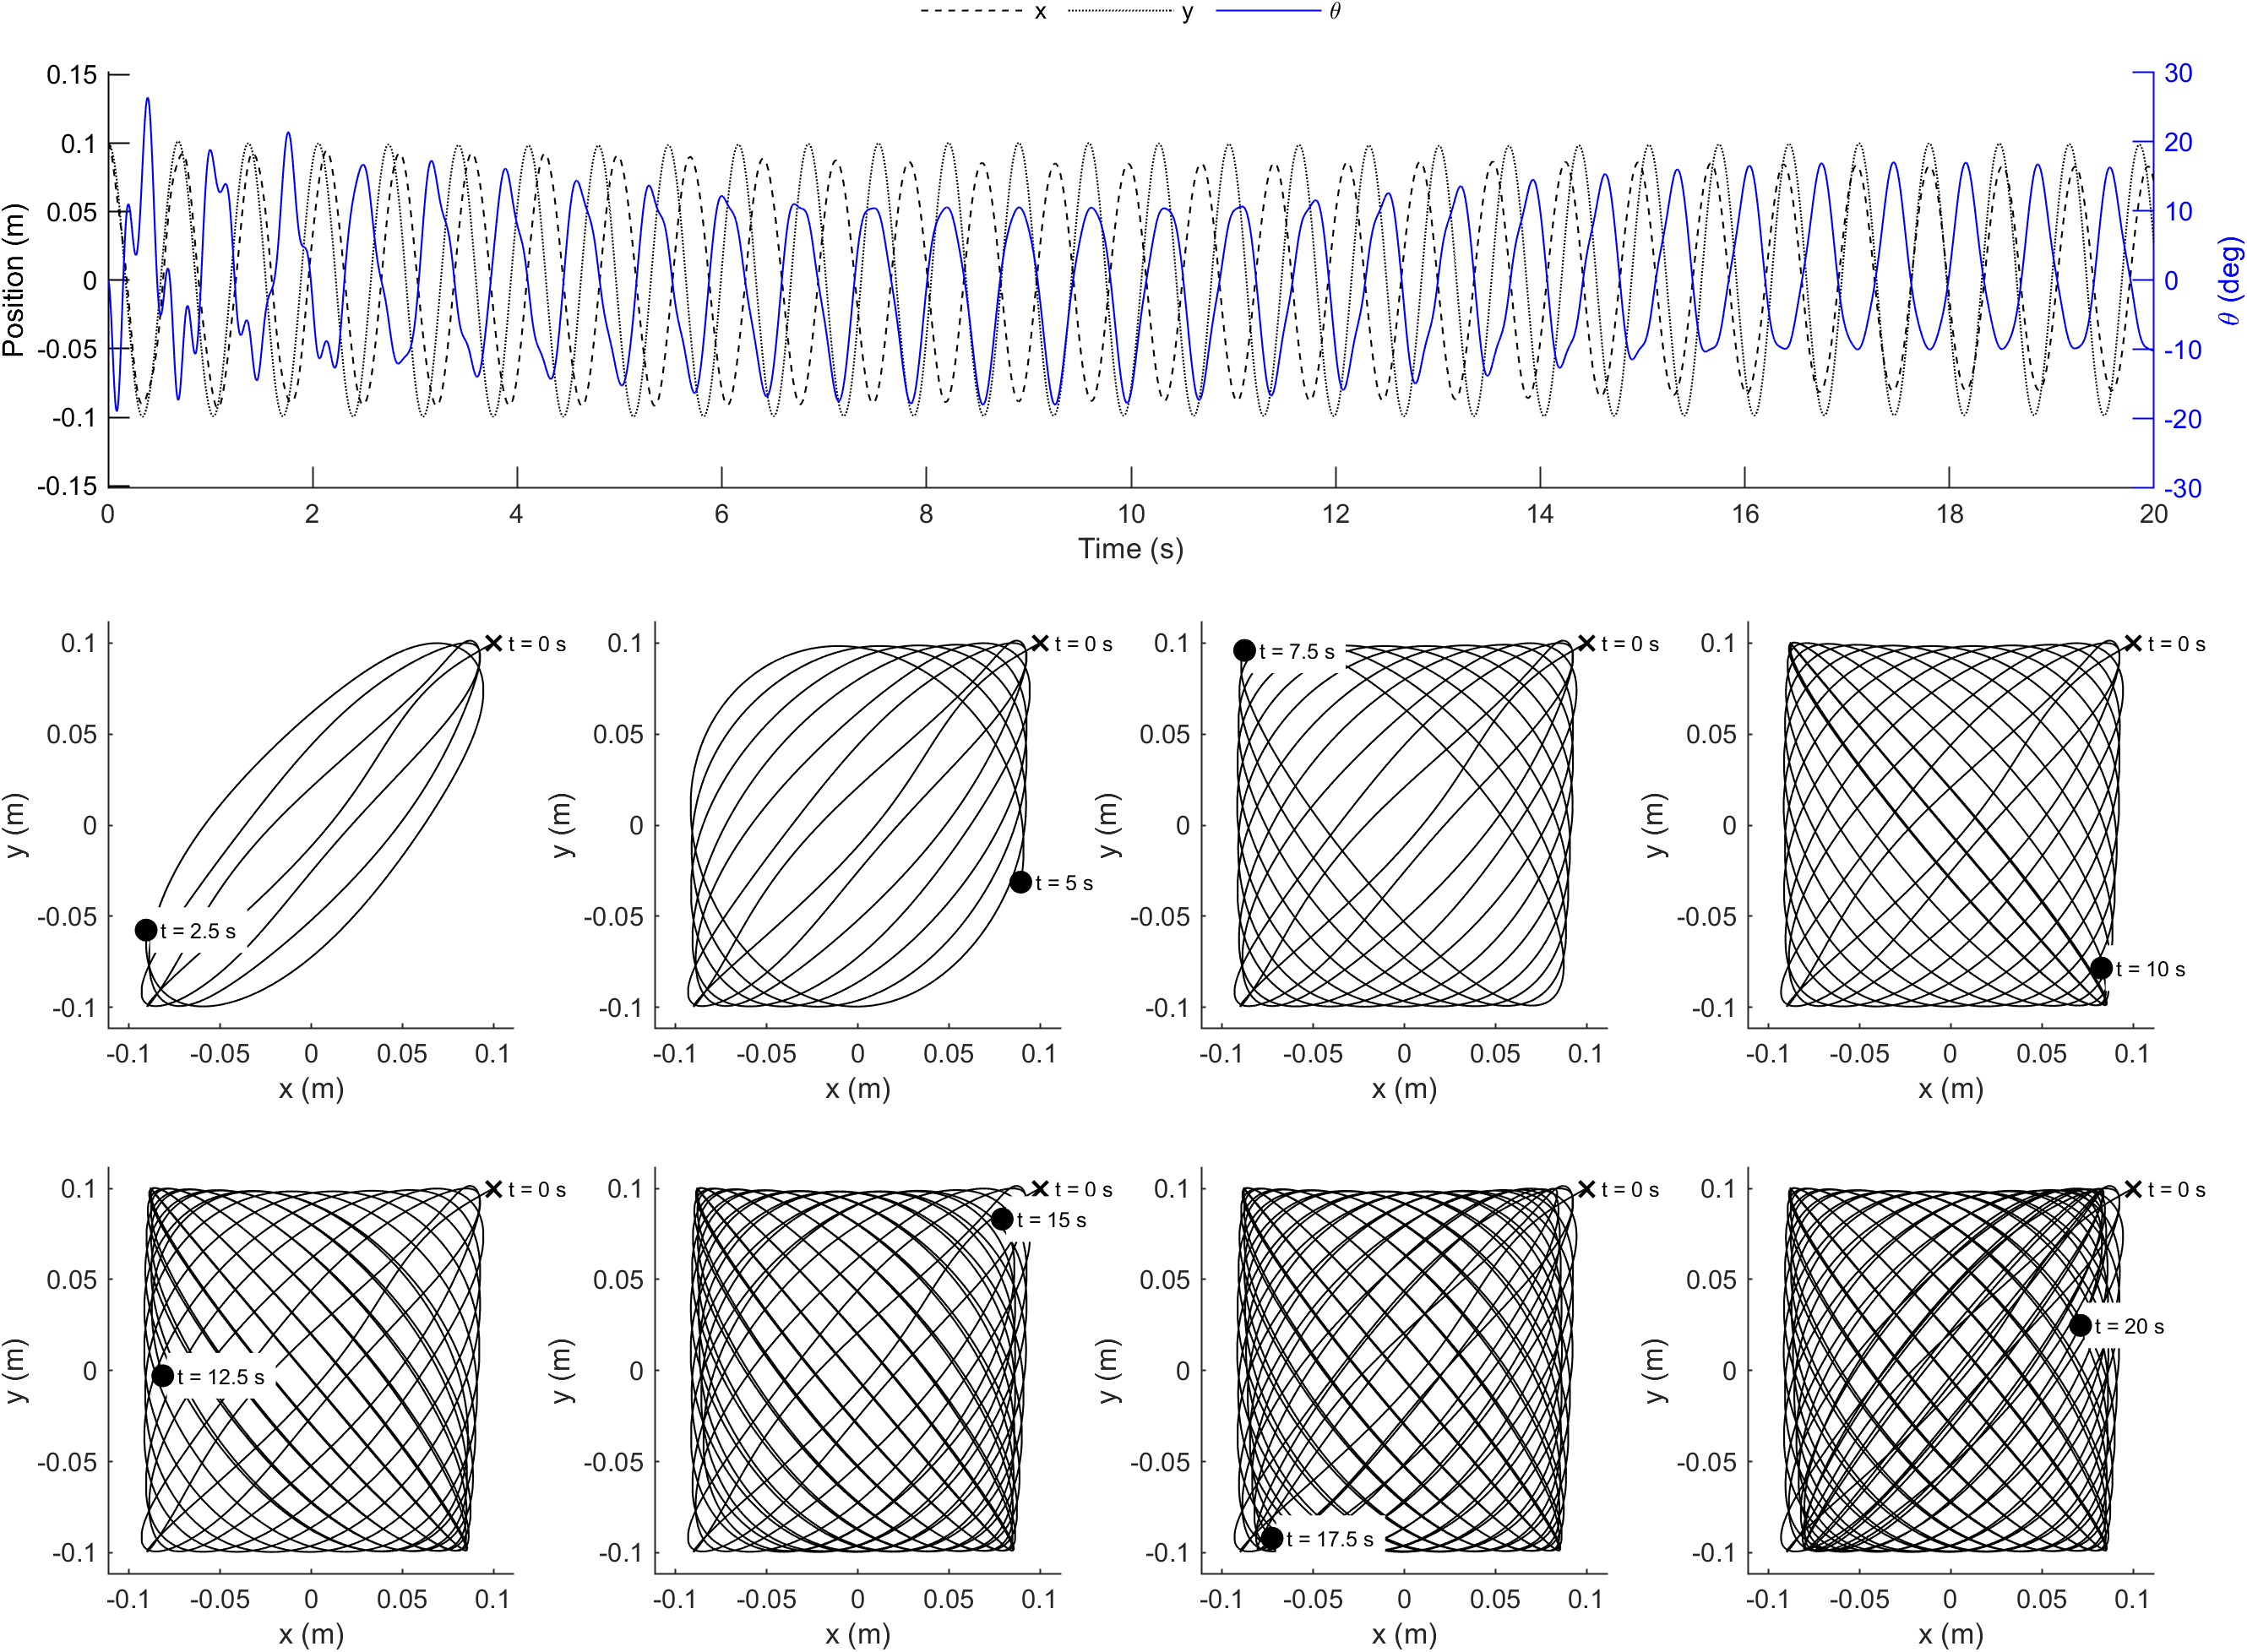
\includegraphics[width=0.7\textwidth]{figures/tabletop.png}
    \caption{Kinematics of the 3 DOF model in the table top configuration.}
    \label{fig:3dof-tabletop}
\end{figure}

\begin{figure}
    \centering
    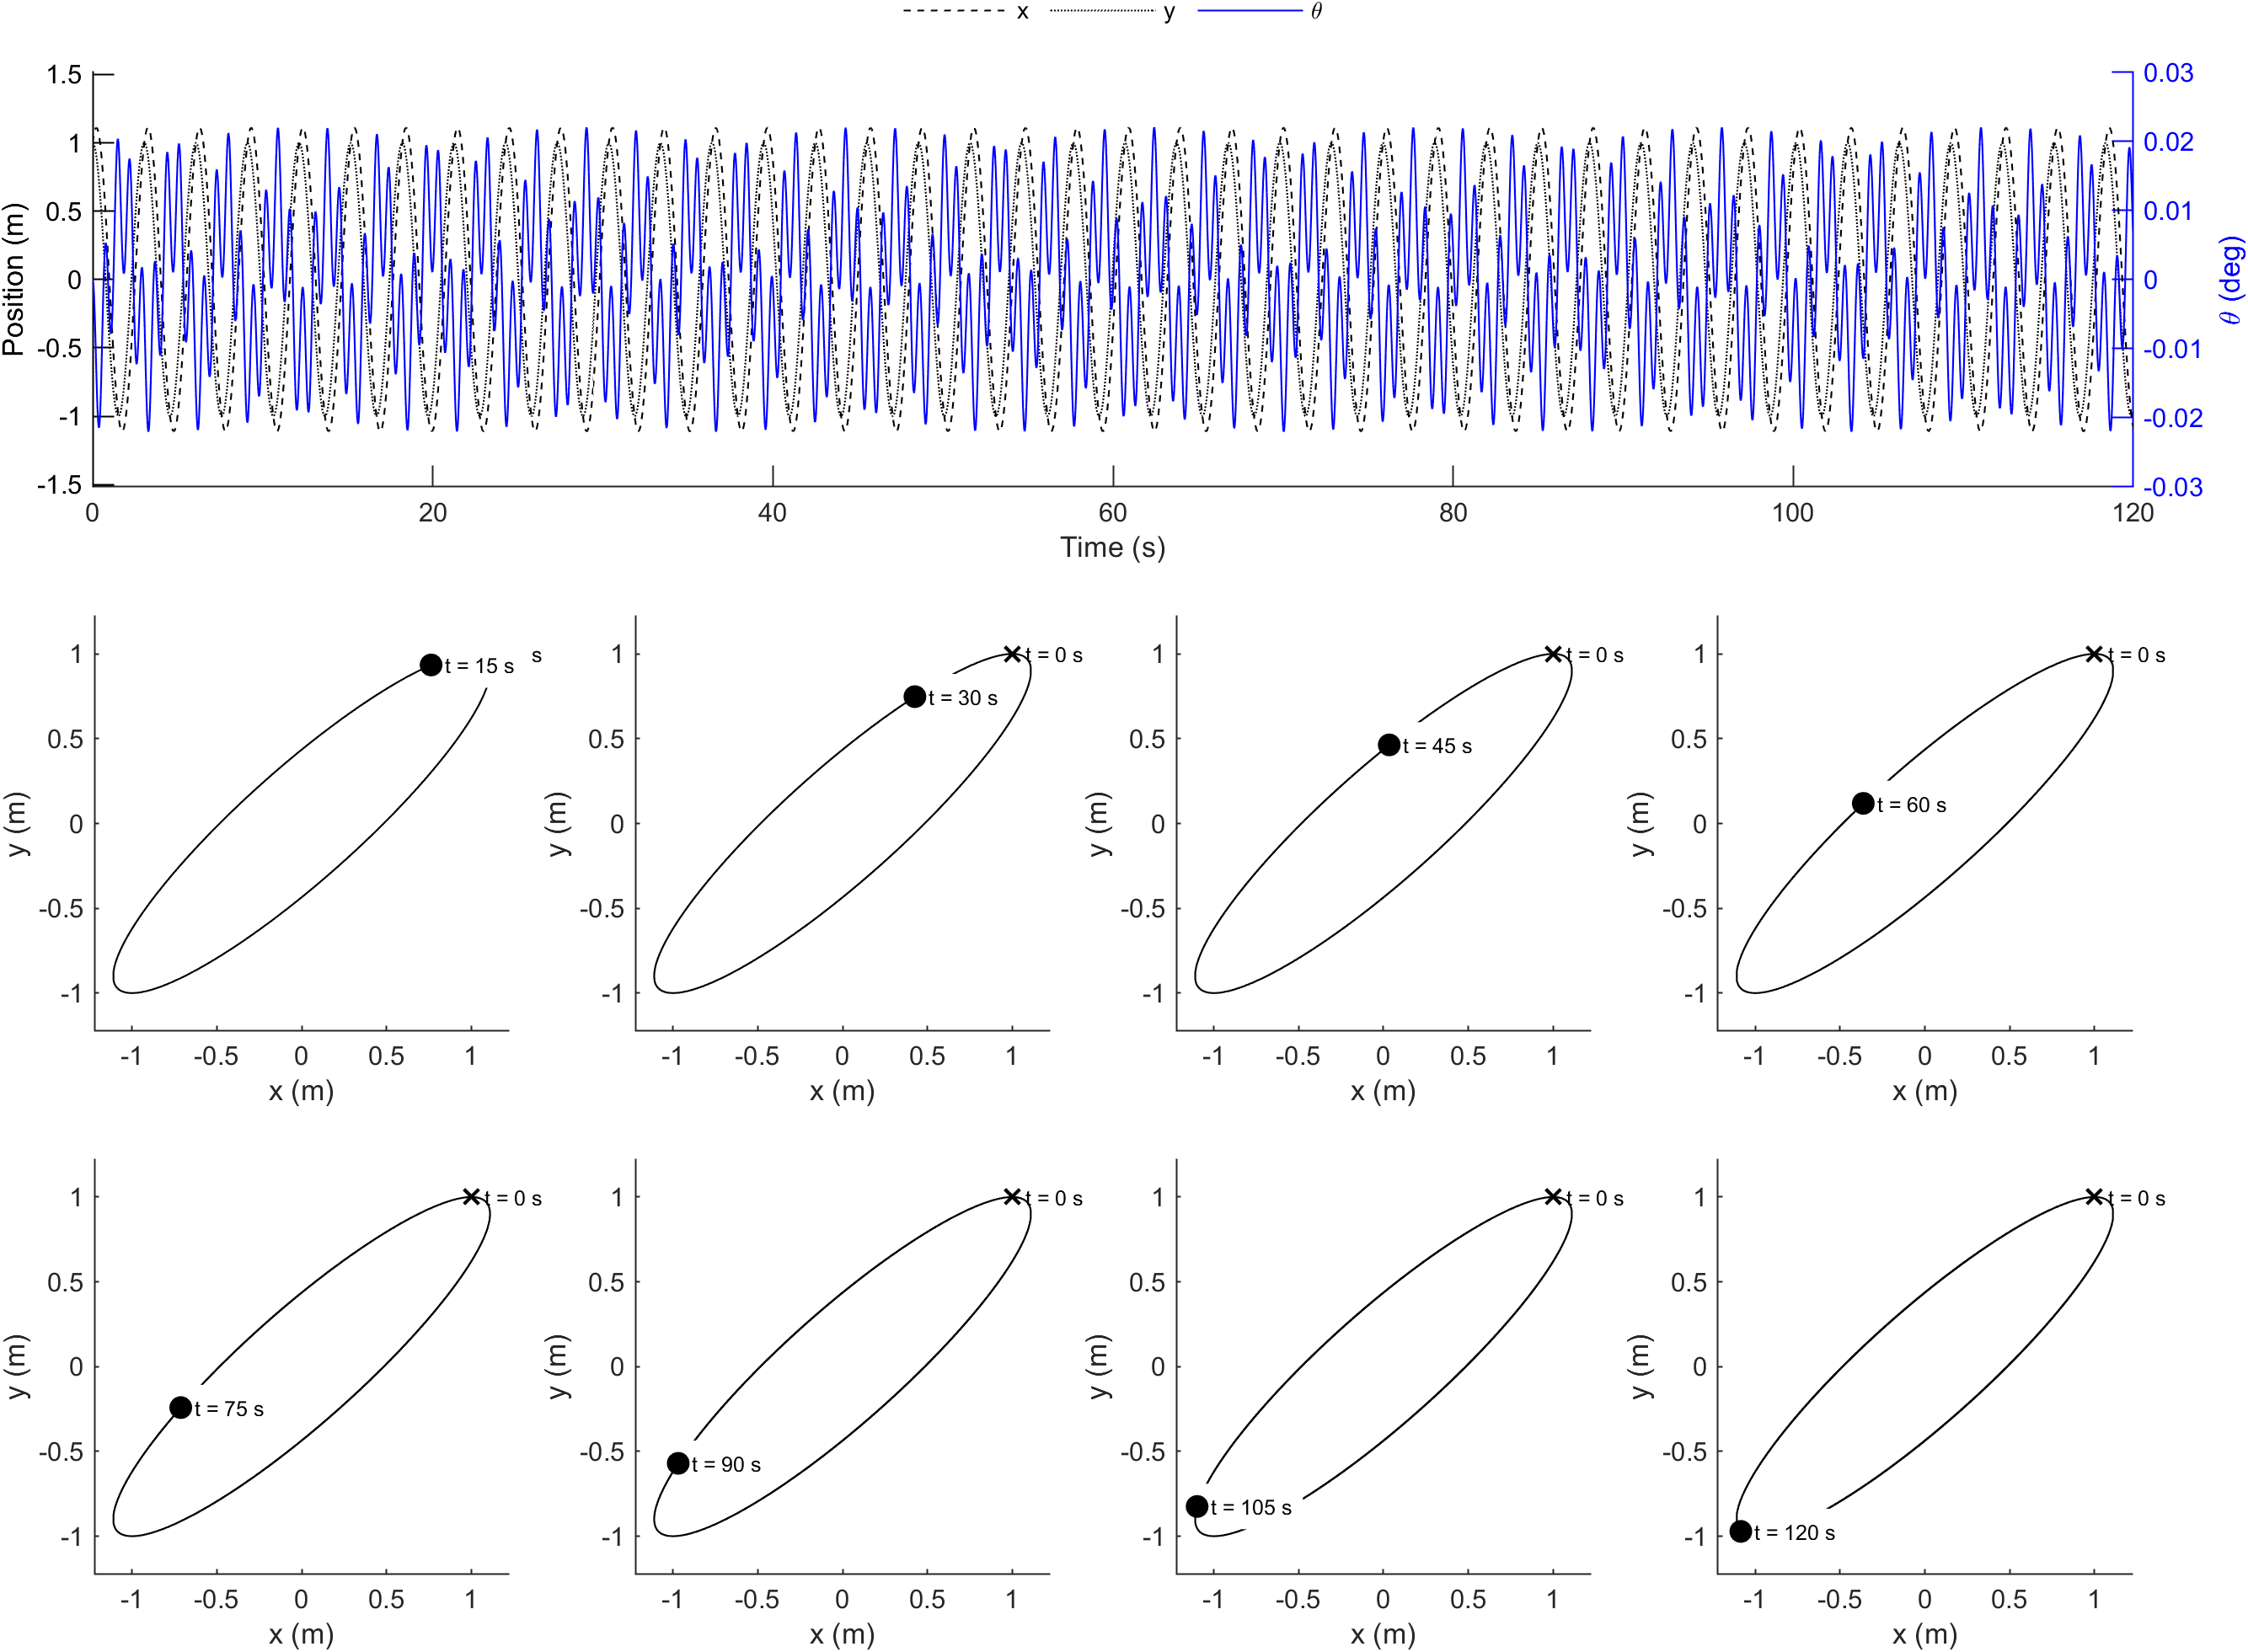
\includegraphics[width=0.7\textwidth]{figures/turbine_typical.png}
    \caption{Kinematics of the 3 DOF model in the typical wind turbine configuration.}
    \label{fig:3dof-turbine-typical}
\end{figure}

\begin{figure}
    \centering
    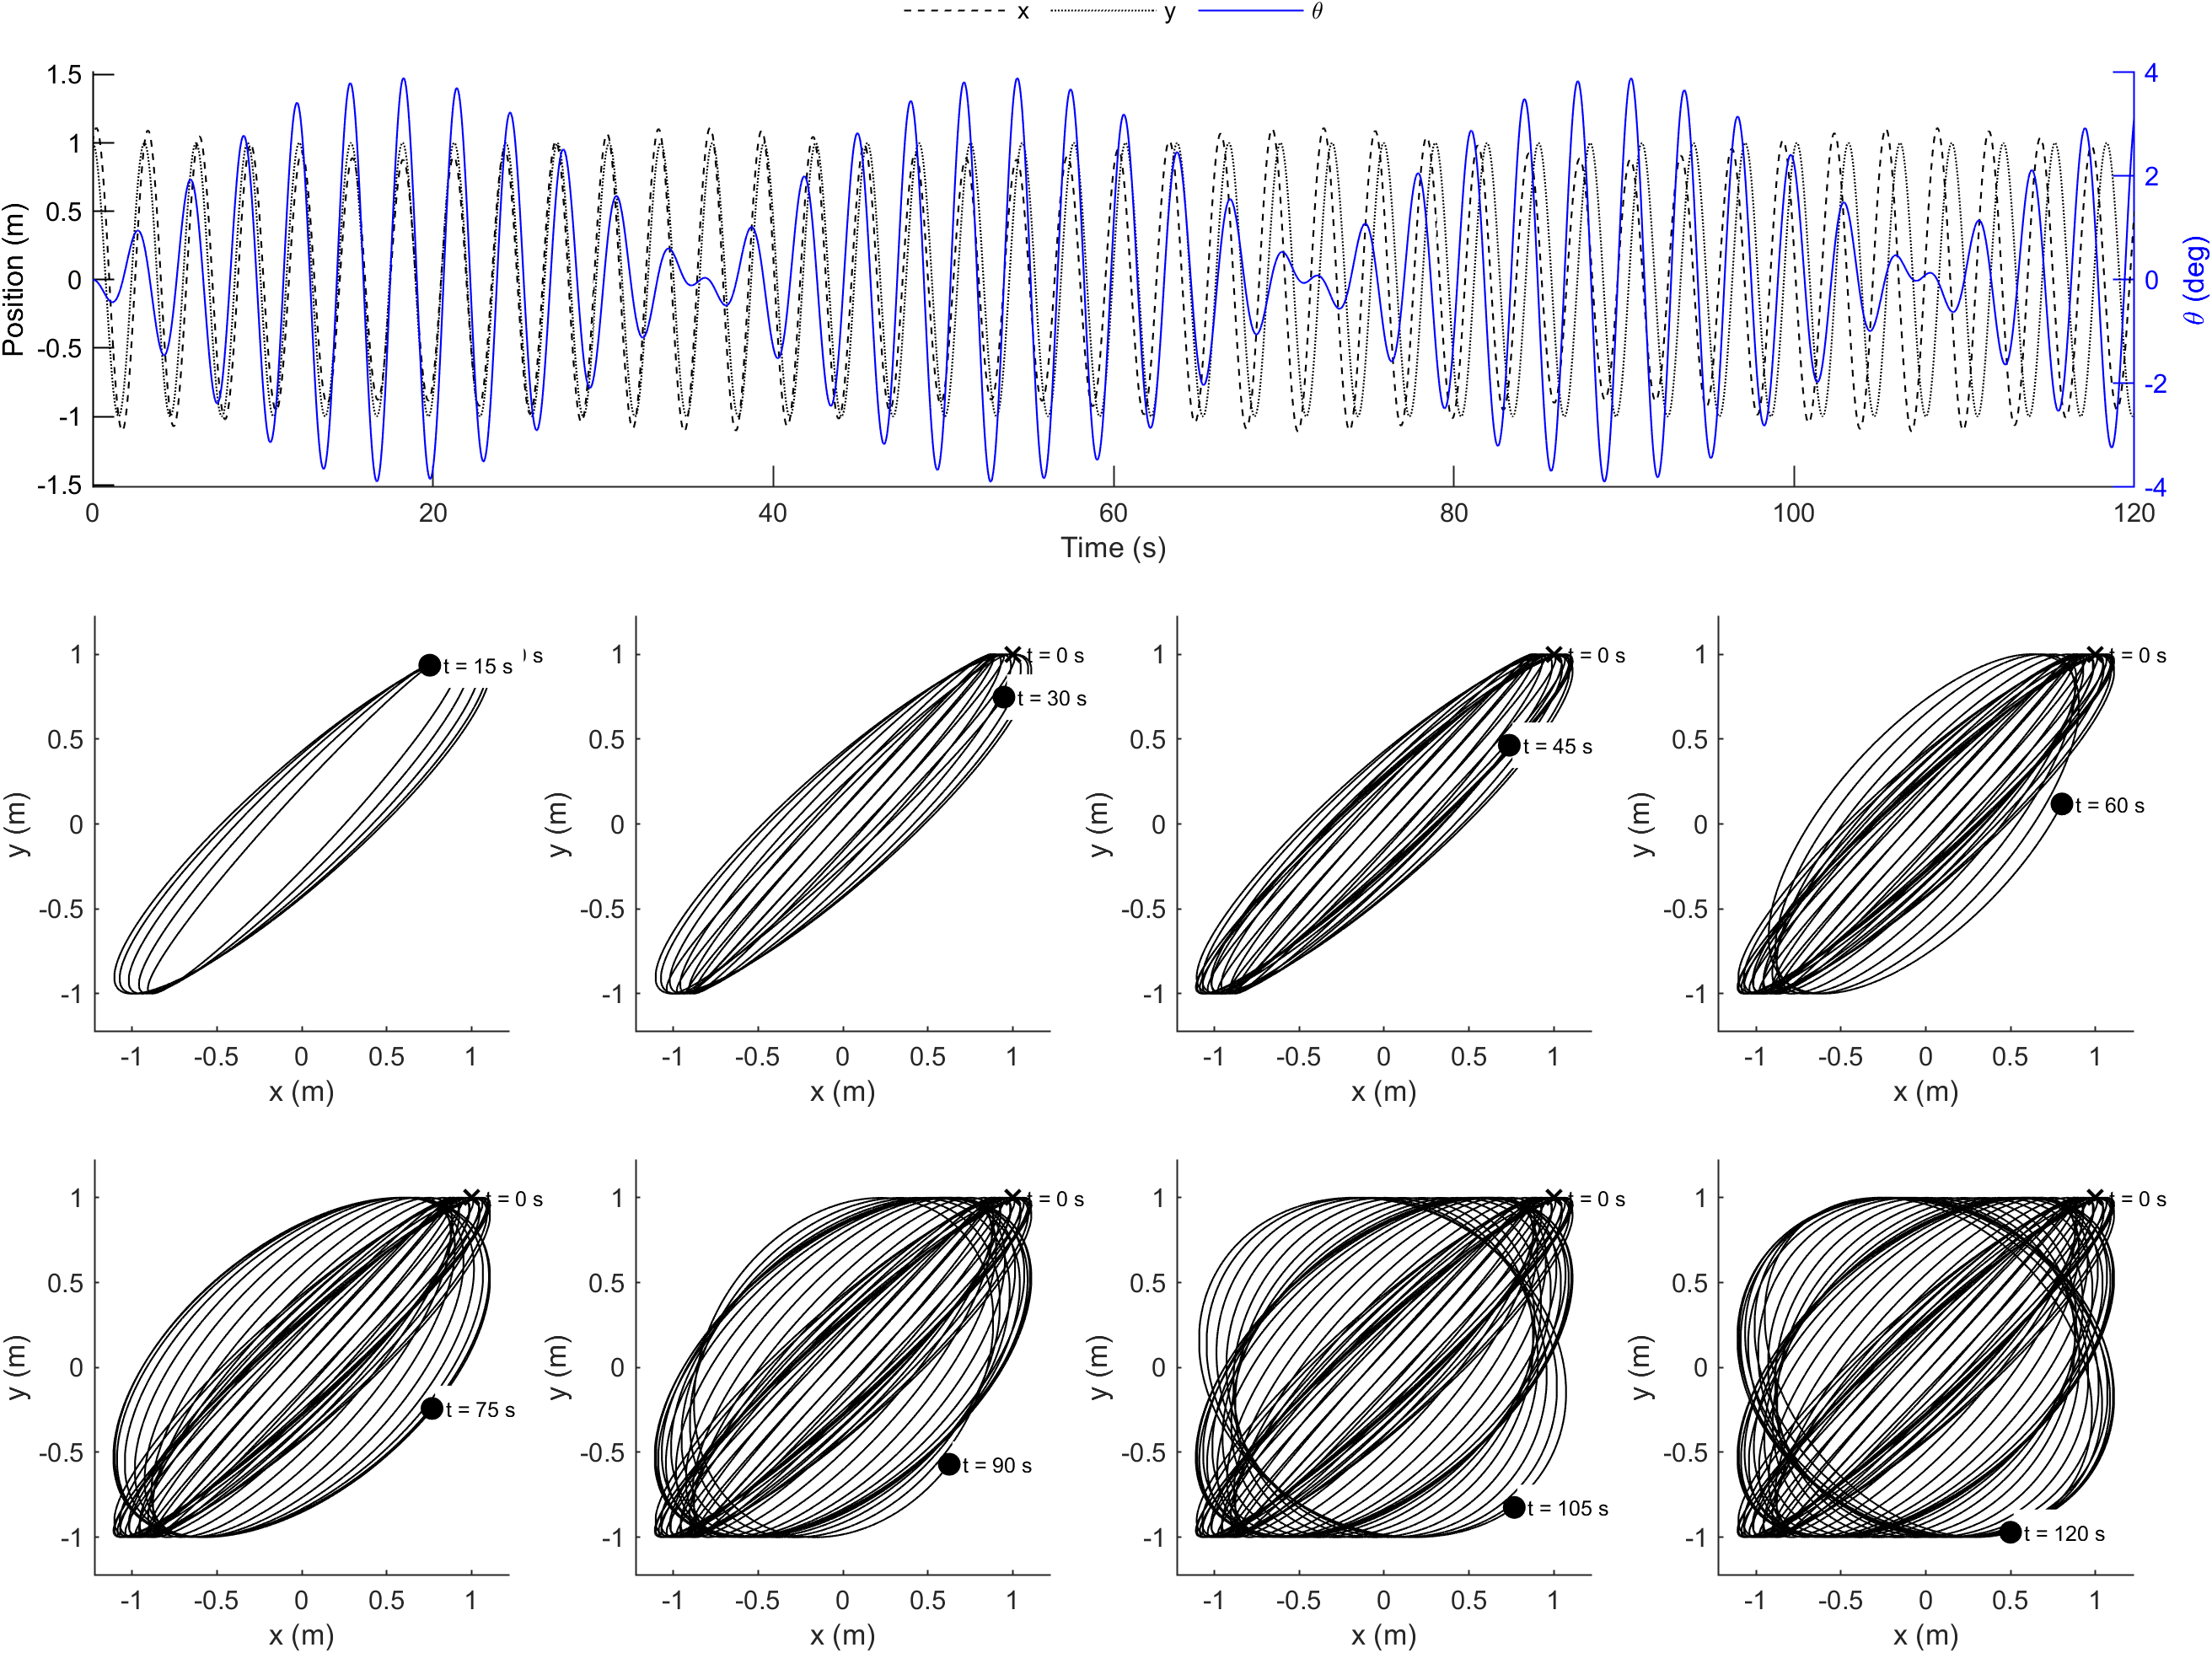
\includegraphics[width=0.7\textwidth]{figures/turbine_unfavorable.png}
    \caption{Kinematics of the 3 DOF model in the unfavorable wind turbine configuration.}
    \label{fig:3dof-turbine-unfavorable}
\end{figure}

\clearpage

\section{Discussion}
\label{sec:discussion}

\subsection{Table-top Experiment}

Even though the table-top experiment was conducted with very limited resources and meant as a demonstrator experiment only, the torsional coupling was clearly observable. More so, the reproducability of the orbits was high, increasing confidence in the effect. In future experiments, more care must be taken to tightly control the initial and boundary conditions of the experiment. It stands to reason, that even without an eccentric mass present at the free end of the rod, orbits will appear in an experiment as simple as ours, given the difficulty of aligning the rod with Earth's gravitational vector and thus always inducing a certain mass eccentricity. In a future study, befor designing a new experiment, the governing parameters should be derived from offshore wind turbines by applying similitude. 

\subsection{Simulation}

With the linear numerical model, similar orbits as observed in the table top experiments have been found. Differences may be due to the fact, that experiments were performed for initial deformations exceeding a linear behaviour, which are not accounted for by the numerical model. However, the similarity between the numerical and experimental results suggest, that the non-linear effects can be neglected. Simulations for load cases with- and without gravitational force and vertical eccentricity of point mass were performed, for eccentricity up to one thirtienth of the height of the cantilevered beam. The effect of  gravitational force and vertical eccentricity appeared negligible. Thereby, it is expected that a simple model with three degrees of freedom, namely translation in both horizontal direction and rotation in the horizontal plane, can be used instead of the rather complex finite element model with six global degrees of freedom. Nevertheless, in future studies, a more realistic model of a partially installed turbine including non-linearities should be investigated as well as more realistic, stochastic loading to determine the full mechanics of the partially installed turbine.

\subsection{3-DoF-Model}

The 3-DoF-model presented in this paper leads to orbits comparable to the table top experiment if the parameters of the differential equations are chosen, such that they are close to the parameters of the table top experiment. However, for parameters resembling an offshore wind turbine no orbits appeared. This needs to be investigated in the future. Furthermore, damping should be added as additional coupling terms between translation and torsion are to be expected if damping is included. A more rigorous mathematical derivation of the 3-DoF-model based on a cantilevered beam formulation should would strengthen the understanding of the torsional couple and would allow to investigate, how realistic the model's assumption of the tower acting as a linear spring is. 

\subsection{Implications for the kinematics of partially installed wind turbines}

So far, a coupling mechanism between translational vibrations sufficient to explain the previously observed orbits in offshore wind turbines undergoing installation has been lacking. The torsional coupling presented here seems to be a valid candidate; however, given the nature of the governing differential equations, it is to be expected that the torsional coupling itself is a highly complex and possibly chaotic effect. Further studies, with parameters closer to real turbines need to be investigated rigorously. It seems, nevertheless, likely, that torsional coupling is present in offshore wind turbines as they are notoriously nose heavy to counter rotor thrust when operational. 

Combining torsional coupling and the stochastic loads inflicted upon the structure by wind and waves may indeed prove to be a sufficient explanation for the formation of orbits during single blade installation.

\clearpage

\bibliographystyle{unsrtnat}
\bibliography{references}  %%% Uncomment this line and comment out the ``thebibliography'' section 

\end{document}
